\documentclass[twocolumn]{aastex631}

\newcommand{\vdag}{(v)^\dagger}
\newcommand\aastex{AAS\TeX}
\newcommand\latex{La\TeX}
\usepackage{amsmath}
\usepackage{multirow}


\begin{document}

\title{Mapping the Diversity of the Black Hole-Stellar Mass Relation Across Cosmological and Feedback Parameter Space}

\author{AstroPilot}
\affiliation{Anthropic, Gemini \& OpenAI servers. Planet Earth.}

\begin{abstract}
The relationship between a galaxy's central black hole mass and its stellar mass is a cornerstone of galaxy evolution, yet the universality of this scaling relation remains an open question. We investigate this by systematically quantifying how the slope, normalization, and scatter of the black hole-stellar mass relation change in response to variations in cosmological parameters and feedback processes. Using a suite of simulated galaxies, where each simulation represents a unique combination of cosmological and feedback parameters, we fit the black hole-stellar mass relation within different stellar mass ranges, focusing on galaxies hosting black holes. We employ multivariate regression and random forest analysis to map how the relation's parameters depend on the input cosmological and feedback parameters. Our results demonstrate that feedback, particularly from supernovae in low-mass galaxies and active galactic nuclei in high-mass galaxies, is the dominant factor driving diversity in the black hole-stellar mass relation. Cosmological parameters influence the normalization and scatter, while the fraction of galaxies hosting black holes is sensitive to feedback, especially in low-mass systems. This work provides a framework for understanding the observed diversity in black hole scaling relations and emphasizes the critical role of feedback in the coevolution of black holes and galaxies.
\
\end{abstract}

\keywords{Black holes, Supermassive black holes, Galaxies, Galaxy evolution, Cosmology, Cosmological parameters, Galaxy clusters, Active galactic nuclei, Feedback, N-body simulations, Gravitational lensing, Galaxy mergers, Galaxy physics, High energy astrophysics, Intergalactic medium}


\section{Introduction}
\label{sec:intro}
The relationship between a galaxy's central supermassive black hole (SMBH) mass and its stellar mass, denoted as $M_{\rm BH}$--$M_{\star}$, stands as a cornerstone in our understanding of galaxy evolution. This scaling relation suggests a co-evolutionary scenario, where the growth of the SMBH is intricately linked to the formation and evolution of its host galaxy. The observed correlation is often interpreted as evidence for feedback mechanisms, whereby energy and momentum injected by the active galactic nucleus (AGN) associated with the SMBH can regulate star formation within the galaxy, and vice versa. However, the universality of this $M_{\rm BH}$--$M_{\star}$ relation remains an open and actively debated question. Observational studies reveal considerable scatter in the relation, and there is growing evidence that the relation may vary depending on galaxy type, environment, and redshift. A comprehensive understanding of the origin and drivers of this diversity is crucial for achieving a complete picture of galaxy evolution.

Establishing a universal $M_{\rm BH}$--$M_{\star}$ relation is challenging for several reasons. Observationally, accurate measurements of black hole masses, especially at high redshifts or in obscured galaxies, are difficult to obtain. Furthermore, stellar mass estimates can also be subject to systematic uncertainties. Theoretically, the complex interplay of various physical processes, such as gas accretion onto the black hole, star formation, and feedback from supernovae (SNe) and AGN, makes it difficult to model the co-evolution of black holes and galaxies. Cosmological parameters may also play a role, influencing the overall structure formation and the assembly histories of galaxies. Disentangling the relative importance of these factors in shaping the $M_{\rm BH}$--$M_{\star}$ relation is a formidable task, requiring a systematic exploration of the parameter space governing galaxy formation and evolution.

In this paper, we tackle the question of the $M_{\rm BH}$--$M_{\star}$ relation's diversity by systematically exploring how the slope, normalization, and scatter of this relation vary in response to changes in both cosmological parameters and feedback processes. We leverage a suite of simulated galaxies, each representing a unique combination of cosmological and feedback parameter values. These simulations provide a controlled environment where we can isolate the impact of individual parameters on the $M_{\rm BH}$--$M_{\star}$ relation. Specifically, we fit the $M_{\rm BH}$--$M_{\star}$ relation, represented as $\log_{10} M_{\rm BH} = \alpha + \beta \log_{10} M_{\star}$, within different stellar mass ranges. We focus on galaxies hosting black holes ($M_{\rm BH} > 0$), excluding galaxies without detected black holes from our primary regression analysis. This approach allows us to concentrate on the scaling relation among galaxies with established SMBHs, while also addressing the black hole occupation fraction separately, providing a more complete picture.

To map the dependence of the $M_{\rm BH}$--$M_{\star}$ relation's parameters (slope $\beta$, normalization $\alpha$, and intrinsic scatter) on the input cosmological and feedback parameters, we employ multivariate regression and random forest analysis. These techniques enable us to quantify the relative importance of each parameter in shaping the scaling relation. Furthermore, we verify our results by examining the black hole occupation fraction as a function of stellar mass and feedback parameters, providing context for the main results and assessing potential selection effects. We also perform secondary analyses to test for residual trends in the $M_{\rm BH}$--$M_{\star}$ relation parameters as a function of star formation rate (SFR), and to quantify the black hole occupation fraction to understand the prevalence of black holes in different galactic environments. By stratifying our analysis across different stellar mass ranges, we account for the varying influence of feedback mechanisms in low-mass versus high-mass galaxies. This comprehensive approach allows us to identify the key physical drivers of diversity in the $M_{\rm BH}$--$M_{\star}$ relation and provides a framework for interpreting observed variations in black hole scaling relations. Our work ultimately aims to provide a more nuanced understanding of the co-evolution of black holes and galaxies by disentangling the complex interplay of cosmological parameters and feedback processes.

\section{Methods}
\label{sec:methods}
\subsection{Simulated Galaxy Data}

Our analysis relies on a suite of simulated galaxies generated from cosmological simulations. Each simulation within the suite is characterized by a unique combination of cosmological parameters and subgrid models for feedback processes. The simulations provide a controlled environment to investigate the impact of these parameters on the black hole-stellar mass relation. The dataset consists of galaxy-level data, including stellar mass ($M_{\star}$), black hole mass ($M_{\rm BH}$), and star formation rate (SFR), along with the corresponding cosmological and feedback parameters for each simulation. The cosmological parameters considered are the matter density ($\Omega_m$) and the amplitude of the matter power spectrum ($\sigma_8$). The feedback parameters control the efficiency of supernova feedback (A\ensuremath{\_}{SN1}, A\ensuremath{\_}{SN2}) and active galactic nuclei feedback (A\ensuremath{\_}{AGN1}, A\ensuremath{\_}{AGN2}). These parameters are systematically varied across the simulation suite, allowing us to explore a wide range of possible galaxy evolution scenarios.

We load the galaxy-level data from a Parquet file (`galaxies_full_optimal.parquet`) and the catalog-level data (containing the cosmological and feedback parameters) from another Parquet file (`catalog_params_optimal.parquet`). We use efficient chunked reading to minimize memory usage, given the large size of the dataset. Each galaxy is associated with its parent catalog's parameters, which are then used as independent variables in our subsequent regression analyses. We only retain the columns that are strictly necessary for the analysis, namely $M_{\star}$, $M_{\rm BH}$, SFR, the catalog number, and the six cosmological/feedback parameters, to further reduce memory footprint and improve computational efficiency.

\subsection{Treatment of Galaxies without Detected Black Holes}

A significant fraction of galaxies, particularly those with low stellar masses, have $M_{\rm BH} = 0$ in the simulation data. These galaxies either do not host a black hole or the black hole mass is below the resolution limit of the simulation. Including these galaxies directly in a log-space regression would introduce a bias, as $\log_{10}(0)$ is undefined. Therefore, we adopt a two-pronged approach to address this issue.

For our primary analysis, which focuses on the scaling relation between $M_{\rm BH}$ and $M_{\star}$, we exclude galaxies with $M_{\rm BH} = 0$ from the regression analysis. This approach is justified by our focus on characterizing the $M_{\rm BH}$--$M_{\star}$ relation among galaxies that *do* host black holes, allowing us to examine the scaling relation without the confounding effect of galaxies lacking detectable black holes. This is further justified by the large sample sizes in each stellar mass bin, ensuring that the regression results are robust even after excluding these galaxies.

In a secondary analysis, we quantify the black hole occupation fraction as a function of stellar mass and feedback parameters. The black hole occupation fraction is defined as the fraction of galaxies within a given stellar mass range that host a black hole with $M_{\rm BH} > 0$. By examining how this fraction varies with stellar mass and feedback parameters, we can gain insights into the conditions that favor black hole formation or growth, and assess potential selection effects arising from excluding galaxies with $M_{\rm BH} = 0$ in our primary analysis.

\subsection{Stratification by Stellar Mass}

To account for the potentially varying influence of feedback mechanisms across different galaxy mass ranges, we stratify our analysis by stellar mass. We divide the galaxies into three stellar mass bins:

\begin{itemize}
    \item Low-mass galaxies: $M_{\star} < 10^9 M_{\odot}$
    \item Intermediate-mass galaxies: $10^9 M_{\odot} \leq M_{\star} < 10^{10} M_{\odot}$
    \item High-mass galaxies: $M_{\star} \geq 10^{10} M_{\odot}$
\end{itemize}

These mass bins are chosen based on the expected dominance of different feedback mechanisms. Supernova feedback is expected to be more important in low-mass galaxies, while AGN feedback is thought to be more significant in high-mass galaxies. This stratification allows us to investigate how the $M_{\rm BH}$--$M_{\star}$ relation is shaped by different feedback processes in different mass regimes.

\subsection{Catalog-Level Regression Analysis}

For each simulation catalog and within each stellar mass bin, we perform an ordinary least squares (OLS) regression to fit the $M_{\rm BH}$--$M_{\star}$ relation. We select galaxies with $M_{\rm BH} > 0$ in each catalog and mass bin and fit the following linear relation in log-space:

$$ \log_{10} M_{\rm BH} = \alpha + \beta \log_{10} M_{\star} $$

where $\alpha$ is the normalization and $\beta$ is the slope of the relation. We record the best-fit values for $\alpha$ and $\beta$, along with the standard deviation of the residuals in log-space, which serves as a measure of the intrinsic scatter in the relation. If the sample size in a given mass bin within a catalog is small (less than 20 galaxies), we flag the regression results as potentially unreliable, as the small sample size may lead to unstable parameter estimates.

\subsection{Mapping Relation Parameters Across Parameter Space}

After performing the regression analysis for each catalog and mass bin, we compile a table containing the following information for each catalog:

\begin{itemize}
    \item Catalog number
    \item Values of the feedback parameters (A\ensuremath{\_}{SN1}, A\ensuremath{\_}{SN2}, A\ensuremath{\_}{AGN1}, A\ensuremath{\_}{AGN2})
    \item Values of the cosmological parameters ($\Omega_m$, $\sigma_8$)
    \item Slope ($\beta$) of the $M_{\rm BH}$--$M_{\star}$ relation in each mass bin
    \item Normalization ($\alpha$) of the $M_{\rm BH}$--$M_{\star}$ relation in each mass bin
    \item Intrinsic scatter of the $M_{\rm BH}$--$M_{\star}$ relation in each mass bin
\end{itemize}

We then use multivariate regression analysis to quantify how the slope, normalization, and scatter of the $M_{\rm BH}$--$M_{\star}$ relation depend on the feedback and cosmological parameters. Specifically, we use multiple linear regression to model each of the relation parameters (slope, normalization, and scatter) as a linear function of the feedback and cosmological parameters. This allows us to estimate the coefficients that quantify the strength and direction of the relationship between each input parameter and the $M_{\rm BH}$--$M_{\star}$ relation parameters.

To assess the relative importance of each parameter in shaping the $M_{\rm BH}$--$M_{\star}$ relation, we use feature importance metrics derived from random forest regression. Random forest regression is a non-parametric method that can capture non-linear relationships and interactions between the input parameters and the target variables (slope, normalization, and scatter). The feature importance metric quantifies the contribution of each input parameter to the predictive power of the random forest model, providing a measure of its relative importance.

\subsection{Secondary Analyses}

In addition to the primary regression analysis, we perform several secondary analyses to further investigate the factors influencing the $M_{\rm BH}$--$M_{\star}$ relation. As described earlier, we compute the black hole occupation fraction for each catalog and mass bin and analyze its dependence on feedback parameters. This provides insights into the prevalence of black holes in different galactic environments and helps to contextualize the results of our primary analysis.

We also test for residual trends in the $M_{\rm BH}$--$M_{\star}$ relation parameters as a function of star formation rate (SFR). Within each mass bin, we use partial correlation analysis to examine the correlation between the $M_{\rm BH}$--$M_{\star}$ relation parameters and SFR, while controlling for the effects of the feedback and cosmological parameters. This allows us to determine whether SFR has an independent influence on the $M_{\rm BH}$--$M_{\star}$ relation, beyond its correlation with the other parameters.

\subsection{Computational Optimization}

Given the computational demands of analyzing a large suite of simulations, we employ several optimization techniques to ensure that our analysis can be completed within a reasonable timeframe. We parallelize the per-catalog regression analyses across multiple CPU cores using the `multiprocessing` library in Python. Since each catalog can be analyzed independently, this embarrassingly parallel computation significantly reduces the overall runtime.

We also use efficient data access methods to minimize memory usage. We load the galaxy data in chunks, rather than loading the entire dataset into memory at once. This reduces the memory footprint and allows us to process larger datasets. We precompute and cache intermediate results, such as galaxy selections for each catalog and mass bin, to avoid redundant computations.

\section{Results}
\label{sec:results}
This section presents the results of our investigation into the diversity of the black hole-stellar mass ($M_{\rm BH}$--$M_{\star}$) relation across a broad range of cosmological and feedback parameter space. We leverage a suite of simulated galaxy catalogs, each characterized by a unique combination of cosmological parameters ($\Omega_m$, $\sigma_8$) and feedback parameters (A\ensuremath{\_}{SN1}, A\ensuremath{\_}{SN2}, A\ensuremath{\_}{AGN1}, A\ensuremath{\_}{AGN2}), enabling a systematic exploration of how the scaling relation's slope, normalization, and scatter respond to changes in the underlying physics. The methodology involves fitting the relation $\log_{10} M_{\rm BH} = \alpha + \beta \log_{10} M_{\star}$ within three stellar mass bins (low: $M_{\star} < 10^9 M_{\odot}$, intermediate: $10^9 M_{\odot} \leq M_{\star} < 10^{10} M_{\odot}$, high: $M_{\star} \geq 10^{10} M_{\odot}$) for each catalog, excluding galaxies with $M_{\rm BH} = 0$ to focus on the scaling among black hole hosts. The resulting best-fit parameters (slope $\beta$, normalization $\alpha$, and intrinsic scatter) are then mapped as functions of the six catalog parameters using multivariate regression and random forest analysis. Additionally, we quantify the black hole occupation fraction as a function of mass and feedback parameters, providing context for the main results and assessing potential selection effects.

\subsection{Diversity of the $M_{\rm BH}$--$M_{\star}$ Relation}

We find significant diversity in the $M_{\rm BH}$--$M_{\star}$ relation across the simulated catalogs. The distributions of the slope ($\beta$), normalization ($\alpha$), and intrinsic scatter vary considerably, particularly in the intermediate and high stellar mass bins.

\subsubsection{Low-mass galaxies ($M_{\star} < 10^9 M_{\odot}$)}

The distribution of slopes ($\beta$) in the low-mass bin exhibits a mean of 0.20 and a standard deviation of 0.09, ranging from -0.07 to 0.58. The normalization ($\alpha$) has a mean of 4.26 with a standard deviation of 0.72, ranging from 1.24 to 6.54. The intrinsic scatter has a mean of 0.11 dex and a standard deviation of 0.05 dex. The mean black hole occupation fraction in this mass bin is 0.72, with a standard deviation of 0.13.

The shallow slope suggests that black hole growth is relatively inefficient or stochastic in these low-mass galaxies. The significant scatter indicates a wide range of black hole masses at a given stellar mass, possibly due to the stochastic nature of star formation and feedback processes in low-mass galaxies. The incomplete occupation fraction suggests that a significant fraction of low-mass galaxies do not host a detectable black hole, potentially due to suppression of black hole formation or growth by supernova feedback.

\begin{figure}[ht!]
    \centering
    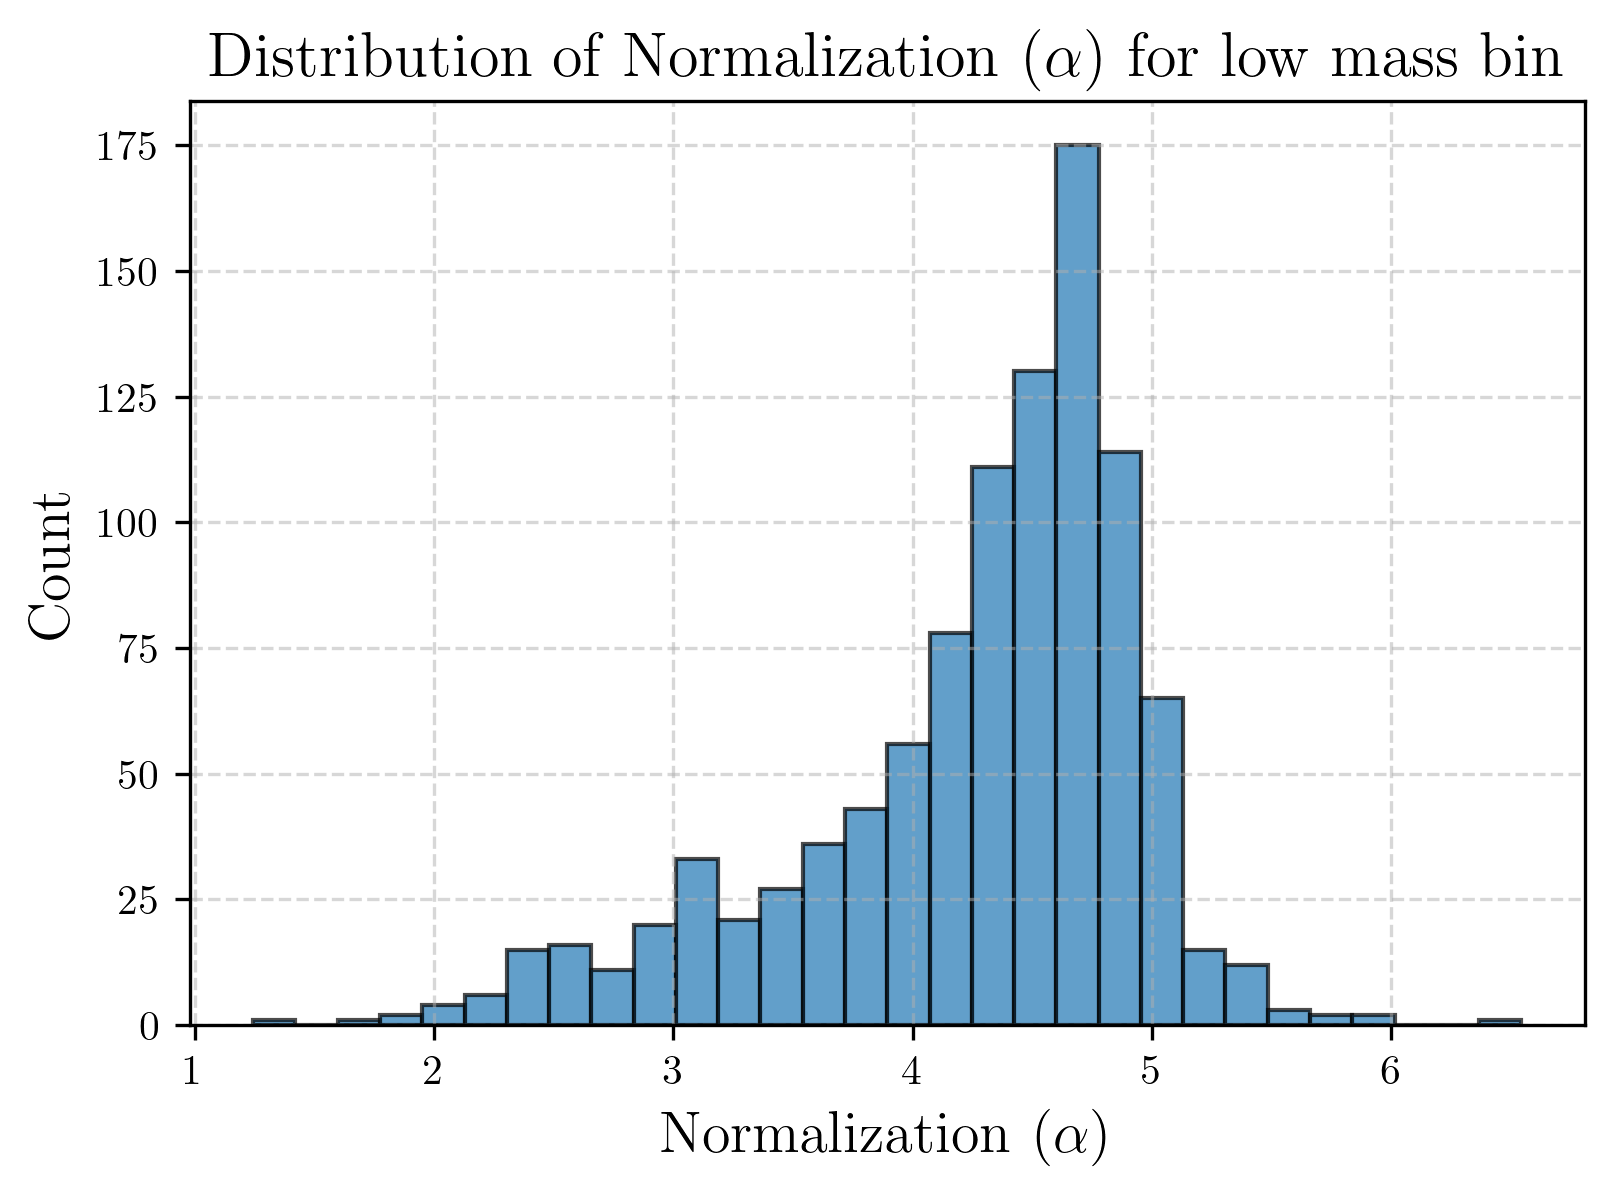
\includegraphics[width=0.5\textwidth]{../Project5/plots/dist_alpha_low_1_20250423_182517.png}
    \caption{Distribution of the normalization parameter $\alpha$ of the $M_\mathrm{BH}$–$M_\mathrm{star}$ relation in the low stellar mass bin ($M_\mathrm{star}<10^9\,M_\odot$) across 1,000 simulated galaxy catalogs, showing the diversity in the relation.
}
    \label{fig:dist_alpha_low}
\end{figure}

\begin{figure}[ht!]
    \centering
    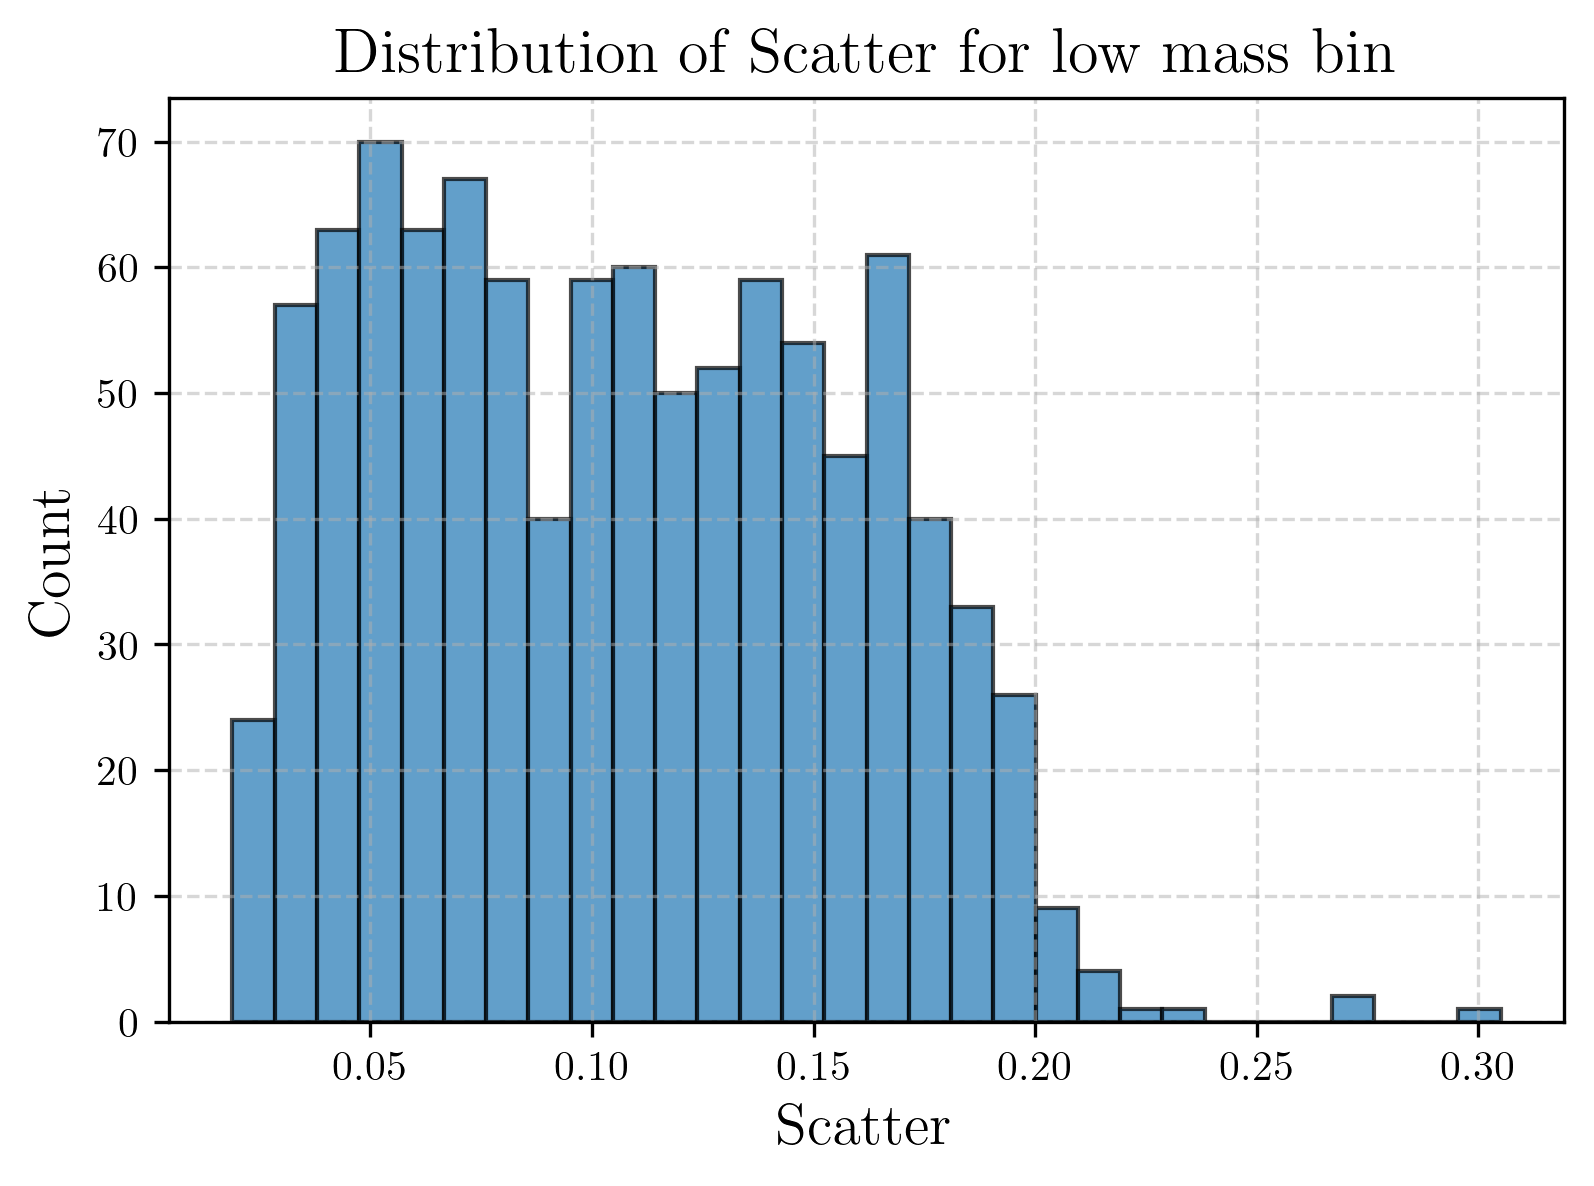
\includegraphics[width=0.5\textwidth]{../Project5/plots/dist_scatter_low_2_20250423_182518.png}
    \caption{Histogram of the intrinsic scatter in the $M_\mathrm{BH}$–$M_\mathrm{star}$ relation for the low stellar mass bin ($M_\mathrm{star}<10^9\,M_\odot$) across 1,000 simulated galaxy catalogs. The distribution reveals a range of scatter values, reflecting the diversity driven by varying feedback and cosmological parameters.
}
    \label{fig:dist_scatter_low}
\end{figure}

\begin{figure}[ht!]
    \centering
    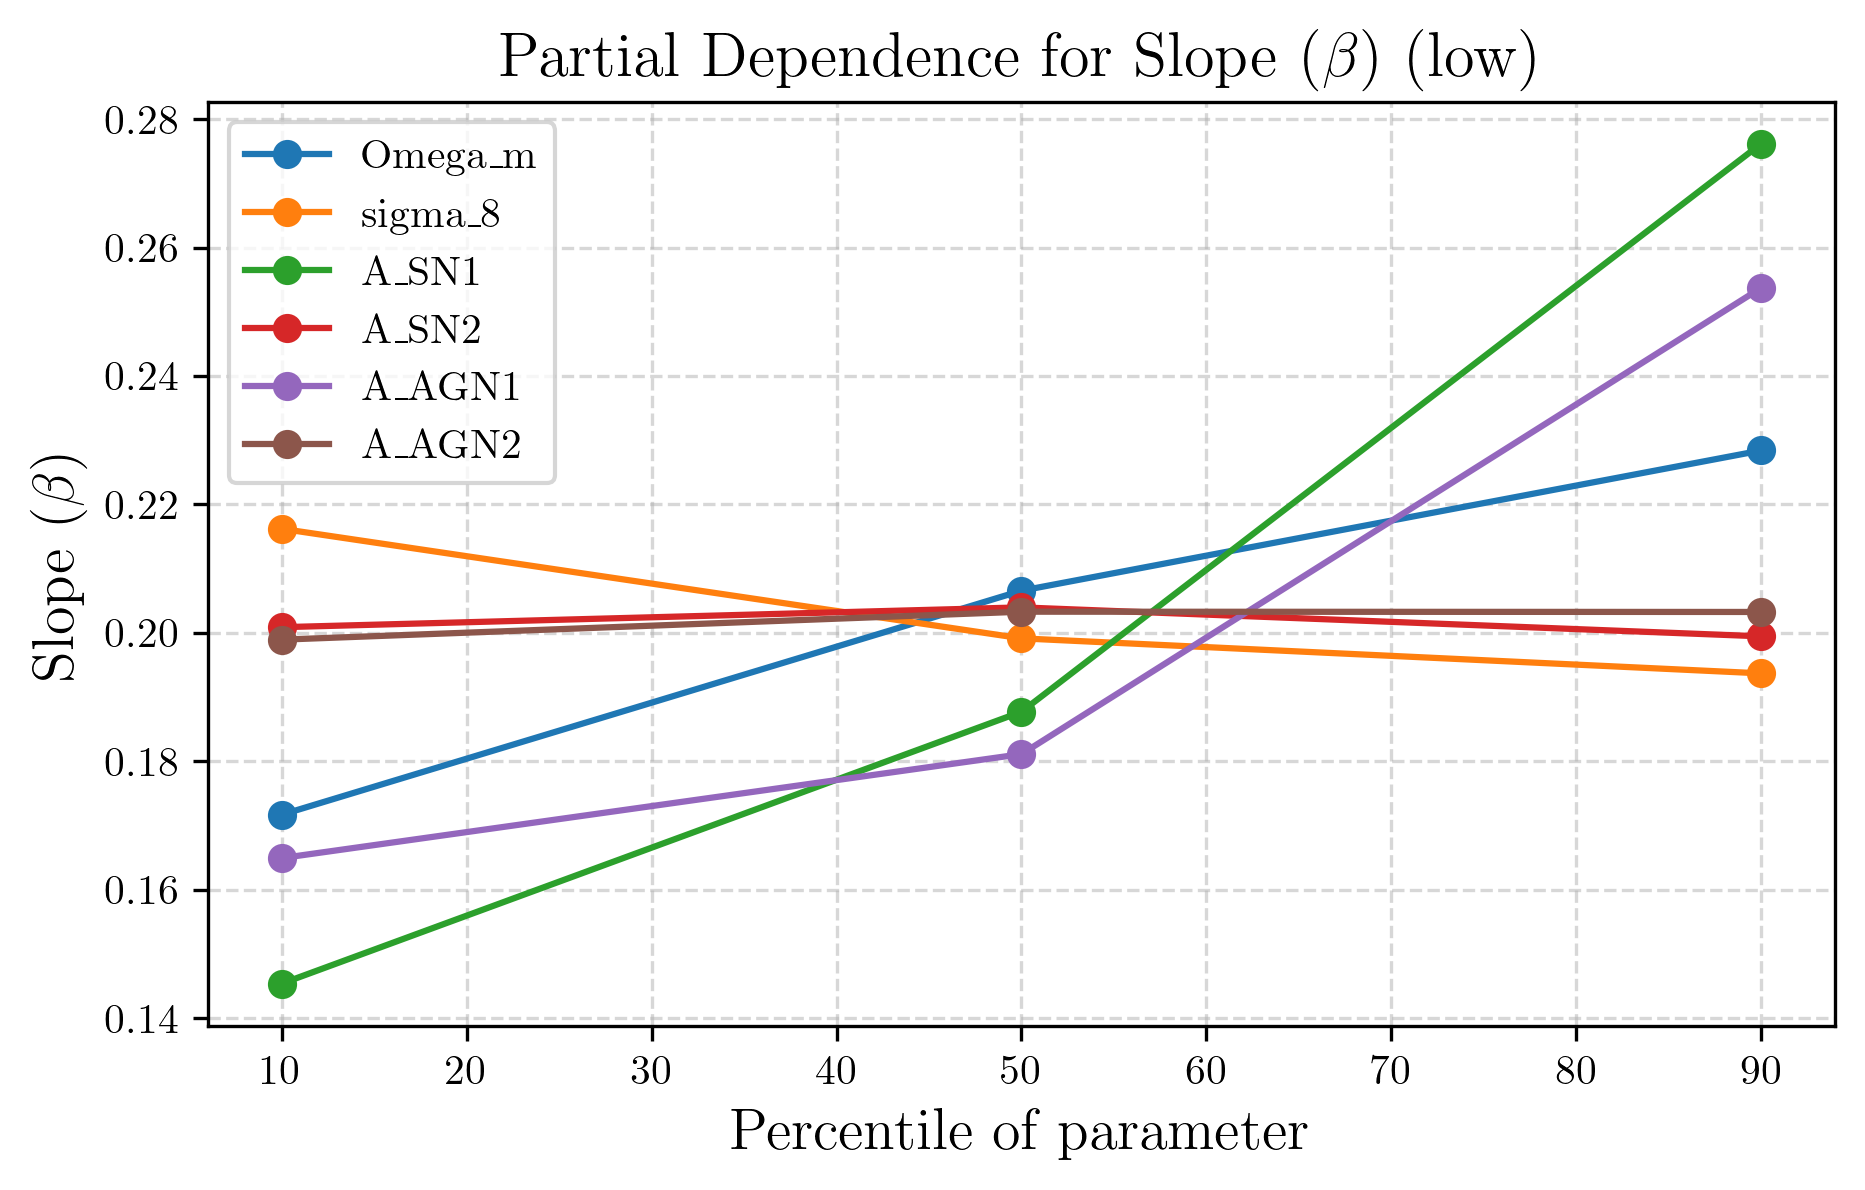
\includegraphics[width=0.5\textwidth]{../Project5/plots/pdp_Slope_beta_low_29_20250423_182536.png}
    \caption{Partial dependence plots showing the effect of varying cosmological ($\Omega_m$, $\sigma_8$) and feedback ($A_{\rm SN1}$, $A_{\rm SN2}$, $A_{\rm AGN1}$, $A_{\rm AGN2}$) parameters on the slope of the $M_{\rm BH}$–$M_{\star}$ relation in the low stellar mass bin. The slope is most sensitive to $A_{\rm SN1}$ and $A_{\rm AGN1}$, indicating the importance of feedback in this regime.
}
    \label{fig:pdp_slope_low}
\end{figure}

\begin{figure}[ht!]
    \centering
    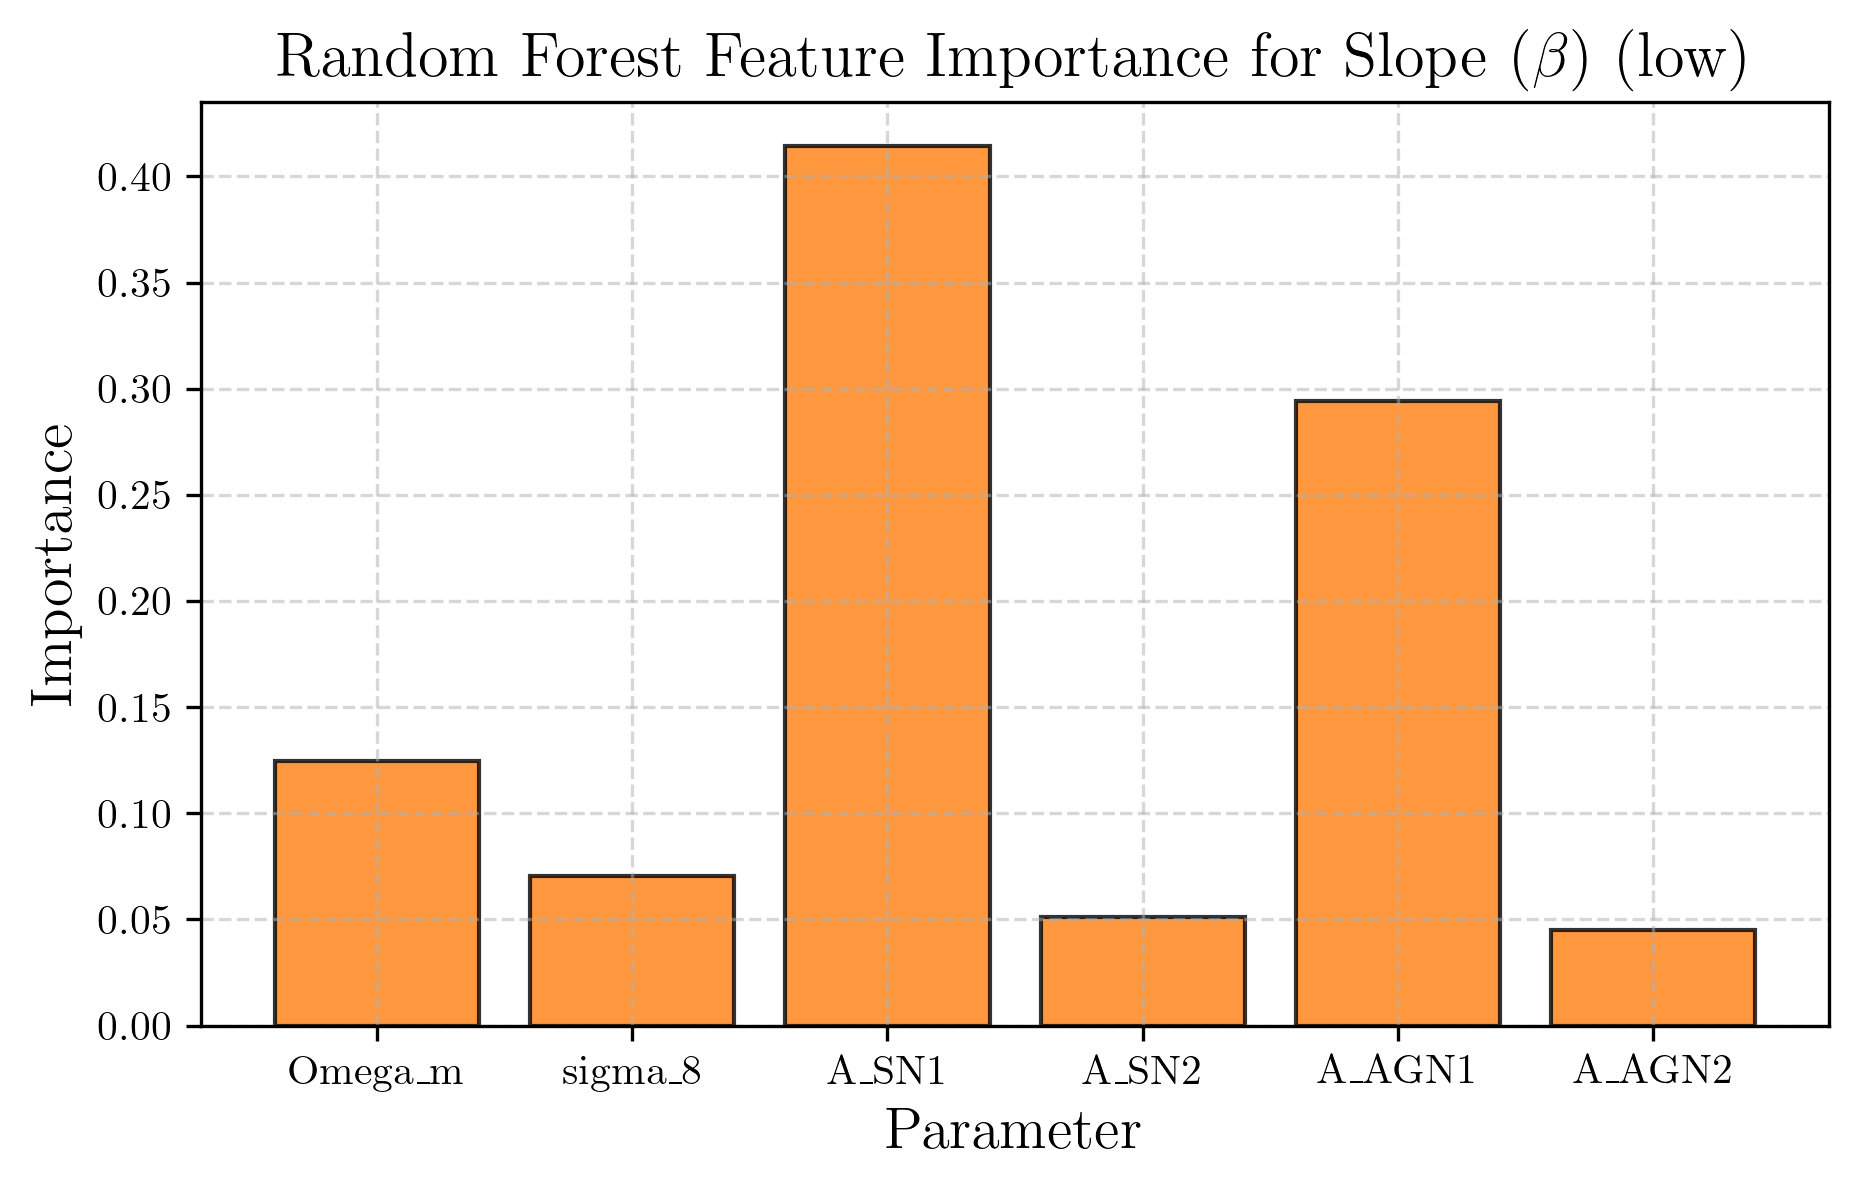
\includegraphics[width=0.5\textwidth]{../Project5/plots/featimp_RandomForest_Slope_beta_low_27_20250423_182532.png}
    \caption{Random forest feature importance for the slope of the black hole stellar mass relation in the low mass bin. The most influential parameters are $A_\mathrm{SN1}$ and $A_\mathrm{AGN1}$, indicating that stronger feedback steepens the relation at low mass.
}
    \label{fig:featimp_slope_low}
\end{figure}

\begin{figure}[ht!]
    \centering
    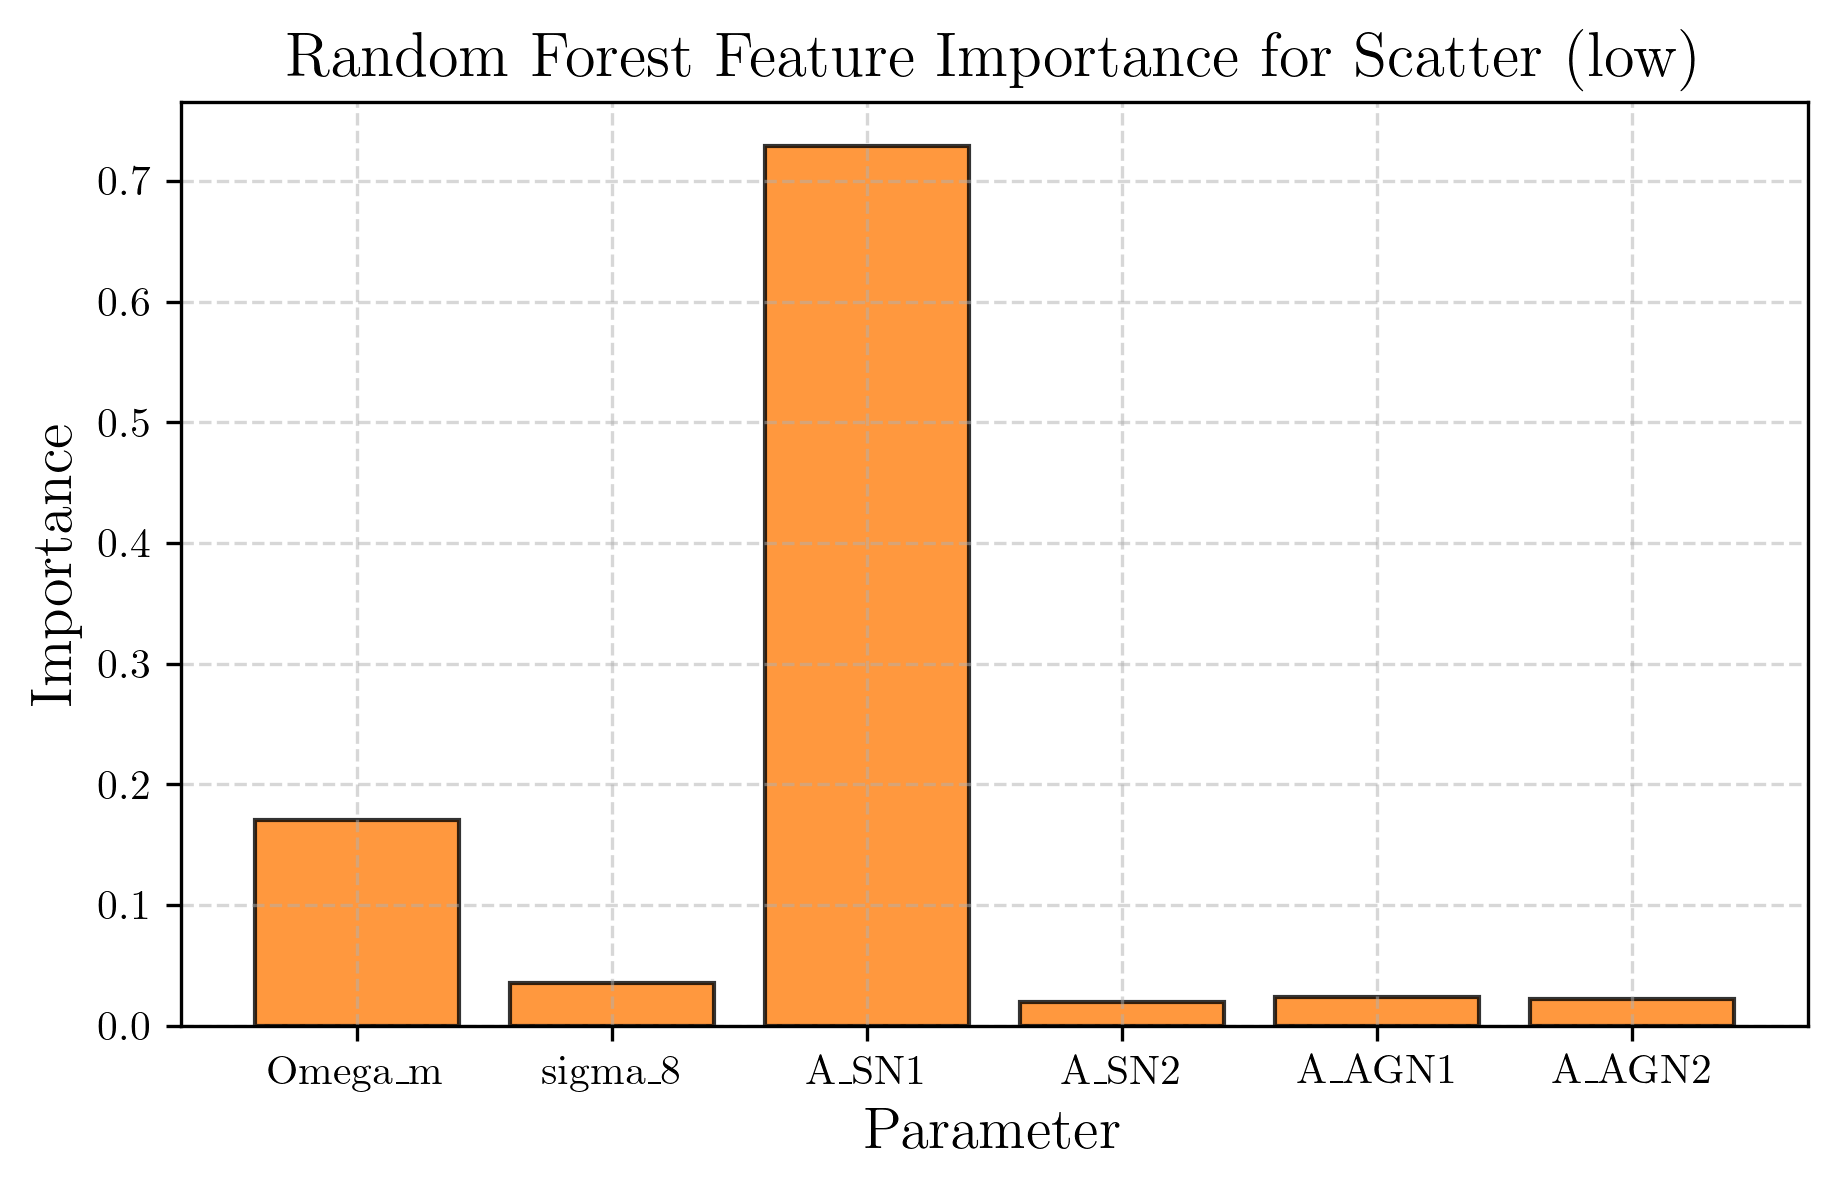
\includegraphics[width=0.5\textwidth]{../Project5/plots/featimp_RandomForest_Scatter_low_33_20250423_182540.png}
    \caption{Random forest feature importance for the scatter in the $M_\mathrm{BH}$–$M_\mathrm{star}$ relation in the low mass bin. Supernova feedback ($A_\mathrm{SN1}$) is the primary driver of increased scatter.
}
    \label{fig:featimp_scatter_random_low}
\end{figure}

\begin{figure}[ht!]
    \centering
    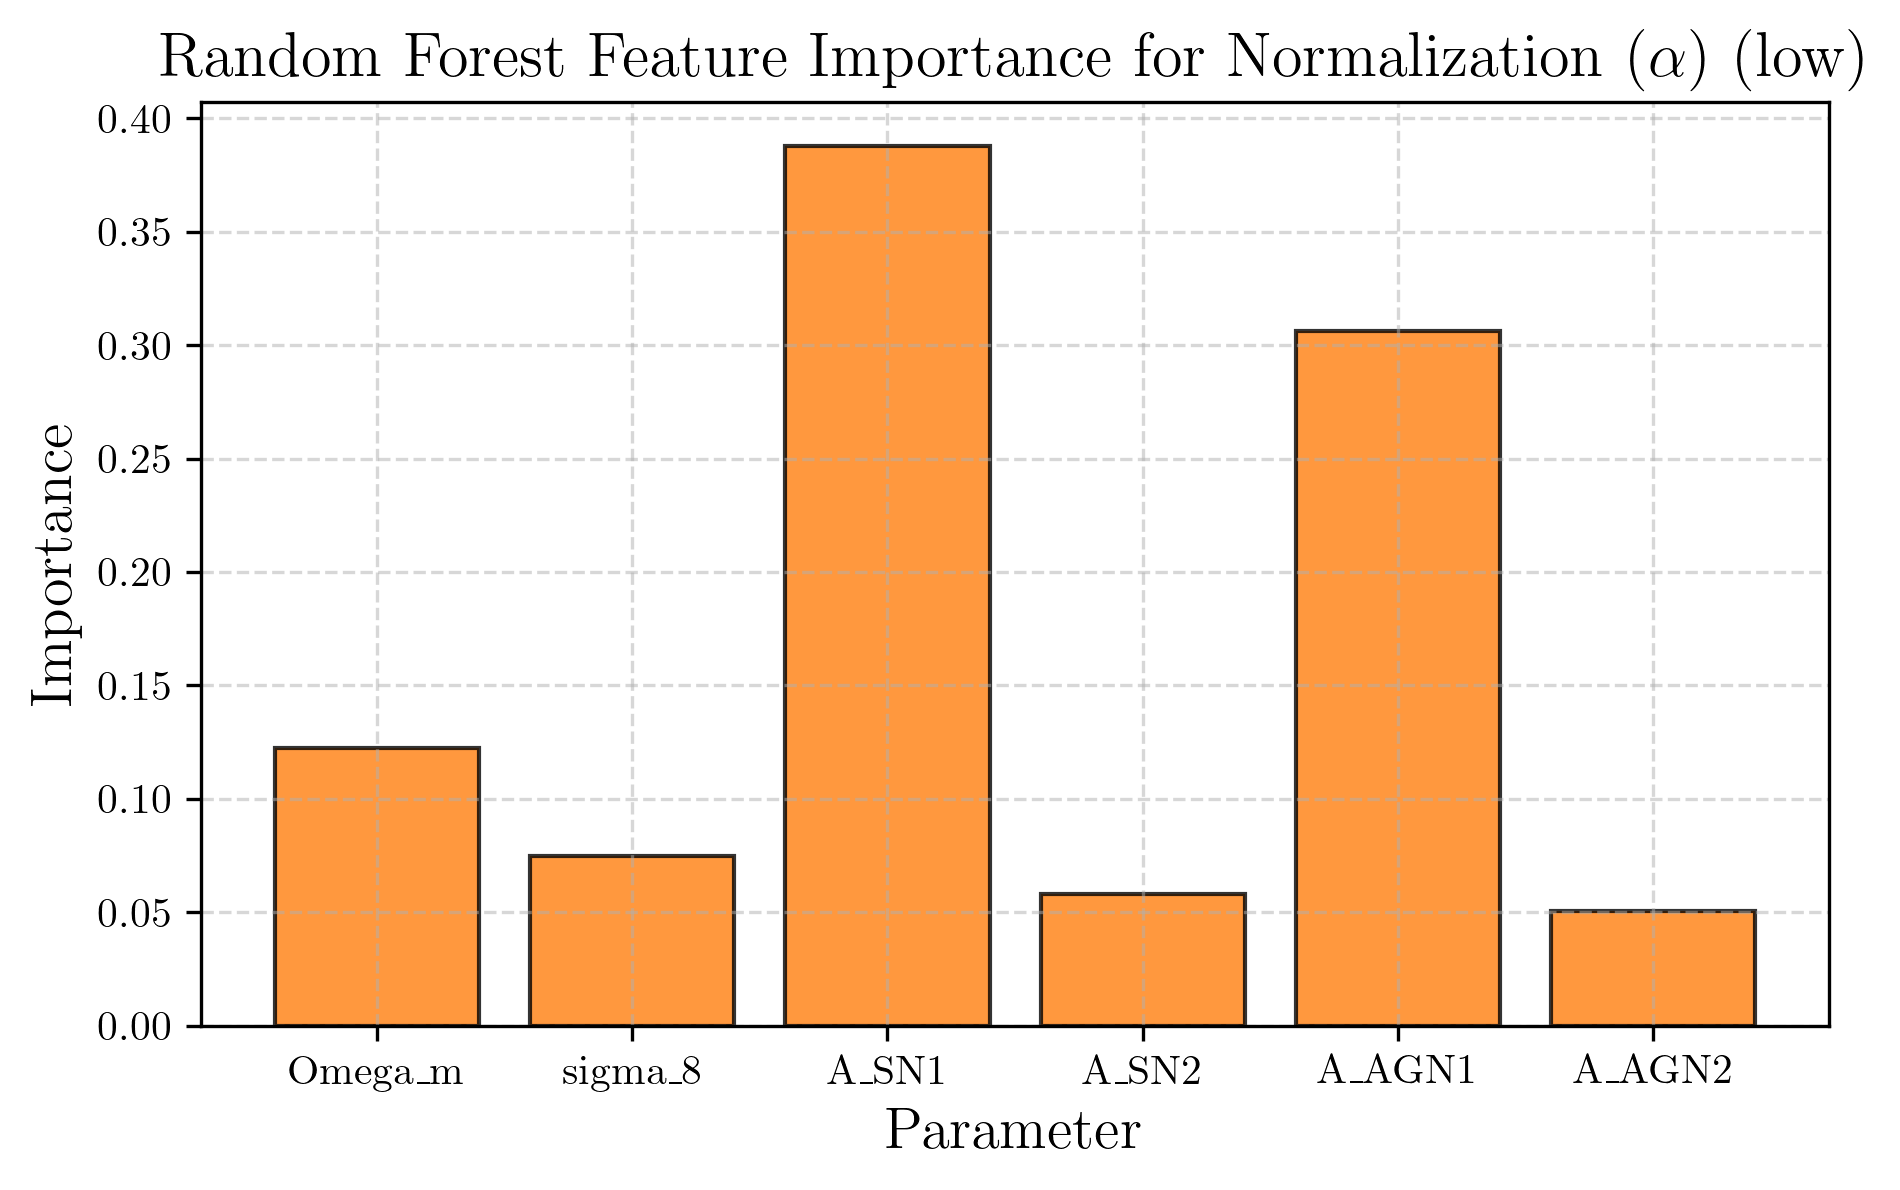
\includegraphics[width=0.5\textwidth]{../Project5/plots/featimp_RandomForest_Normalization_alpha_low_30_20250423_182538.png}
    \caption{Random forest feature importance for the normalization of the $M_{\rm BH}$–$M_{\star}$ relation ($\alpha$) in the low mass bin ($M_{\star}<10^9\,M_\odot$). The bar plot indicates that $A_{\rm SN1}$ and $A_{\rm AGN1}$ are the most important parameters in determining the normalization.
}
    \label{fig:featimp_norm_low}
\end{figure}

\begin{figure}[ht!]
    \centering
    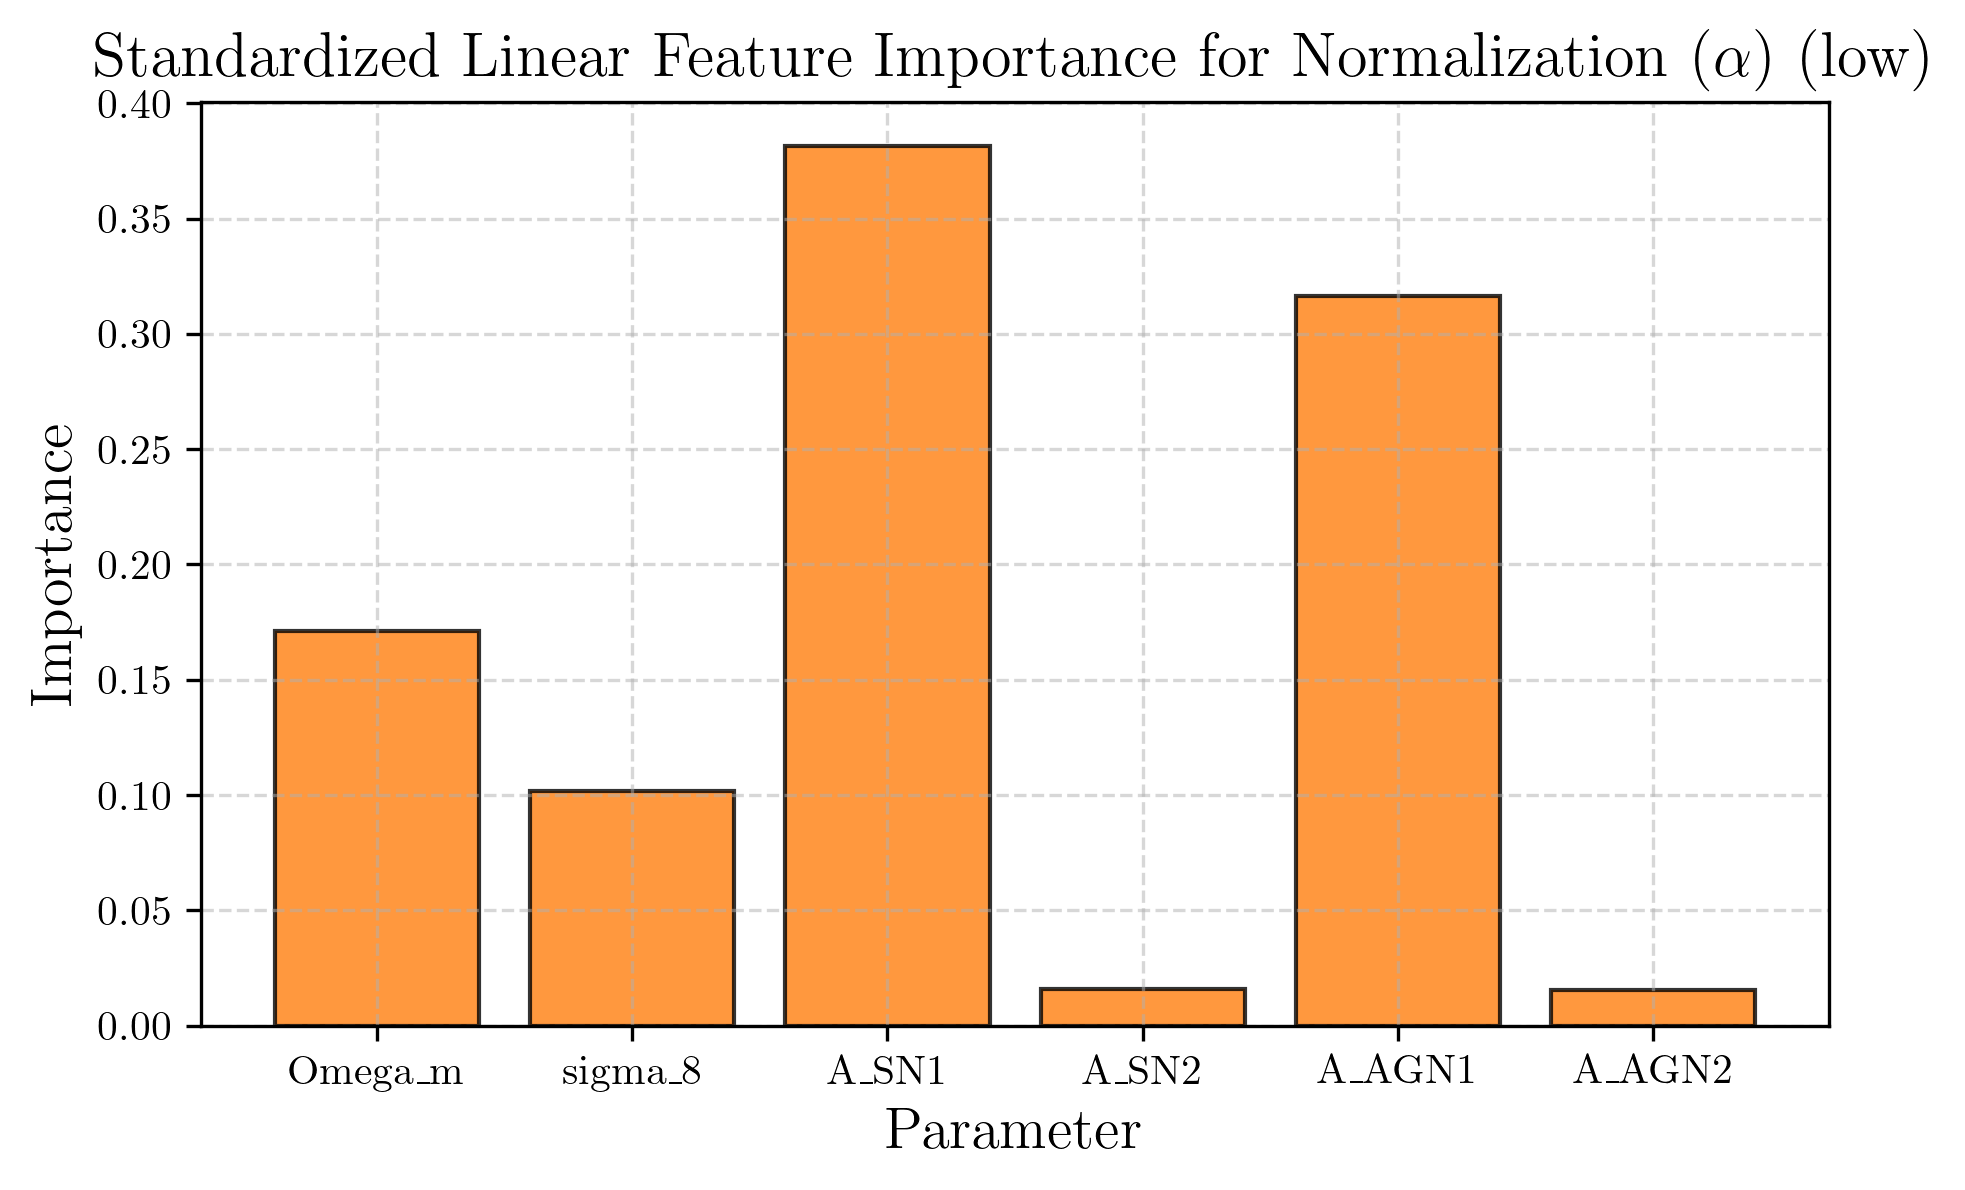
\includegraphics[width=0.5\textwidth]{../Project5/plots/featimp_StandardizedLinear_Normalization_alpha_low_31_20250423_182539.png}
    \caption{Standardized linear regression feature importance for the normalization of the black hole - stellar mass relation in the low stellar mass bin. Supernova feedback ($A_\mathrm{SN1}$) and AGN feedback ($A_\mathrm{AGN1}$) are the most important parameters.
}
    \label{fig:featimp_norm_linear_low}
\end{figure}

\begin{figure}[ht!]
    \centering
    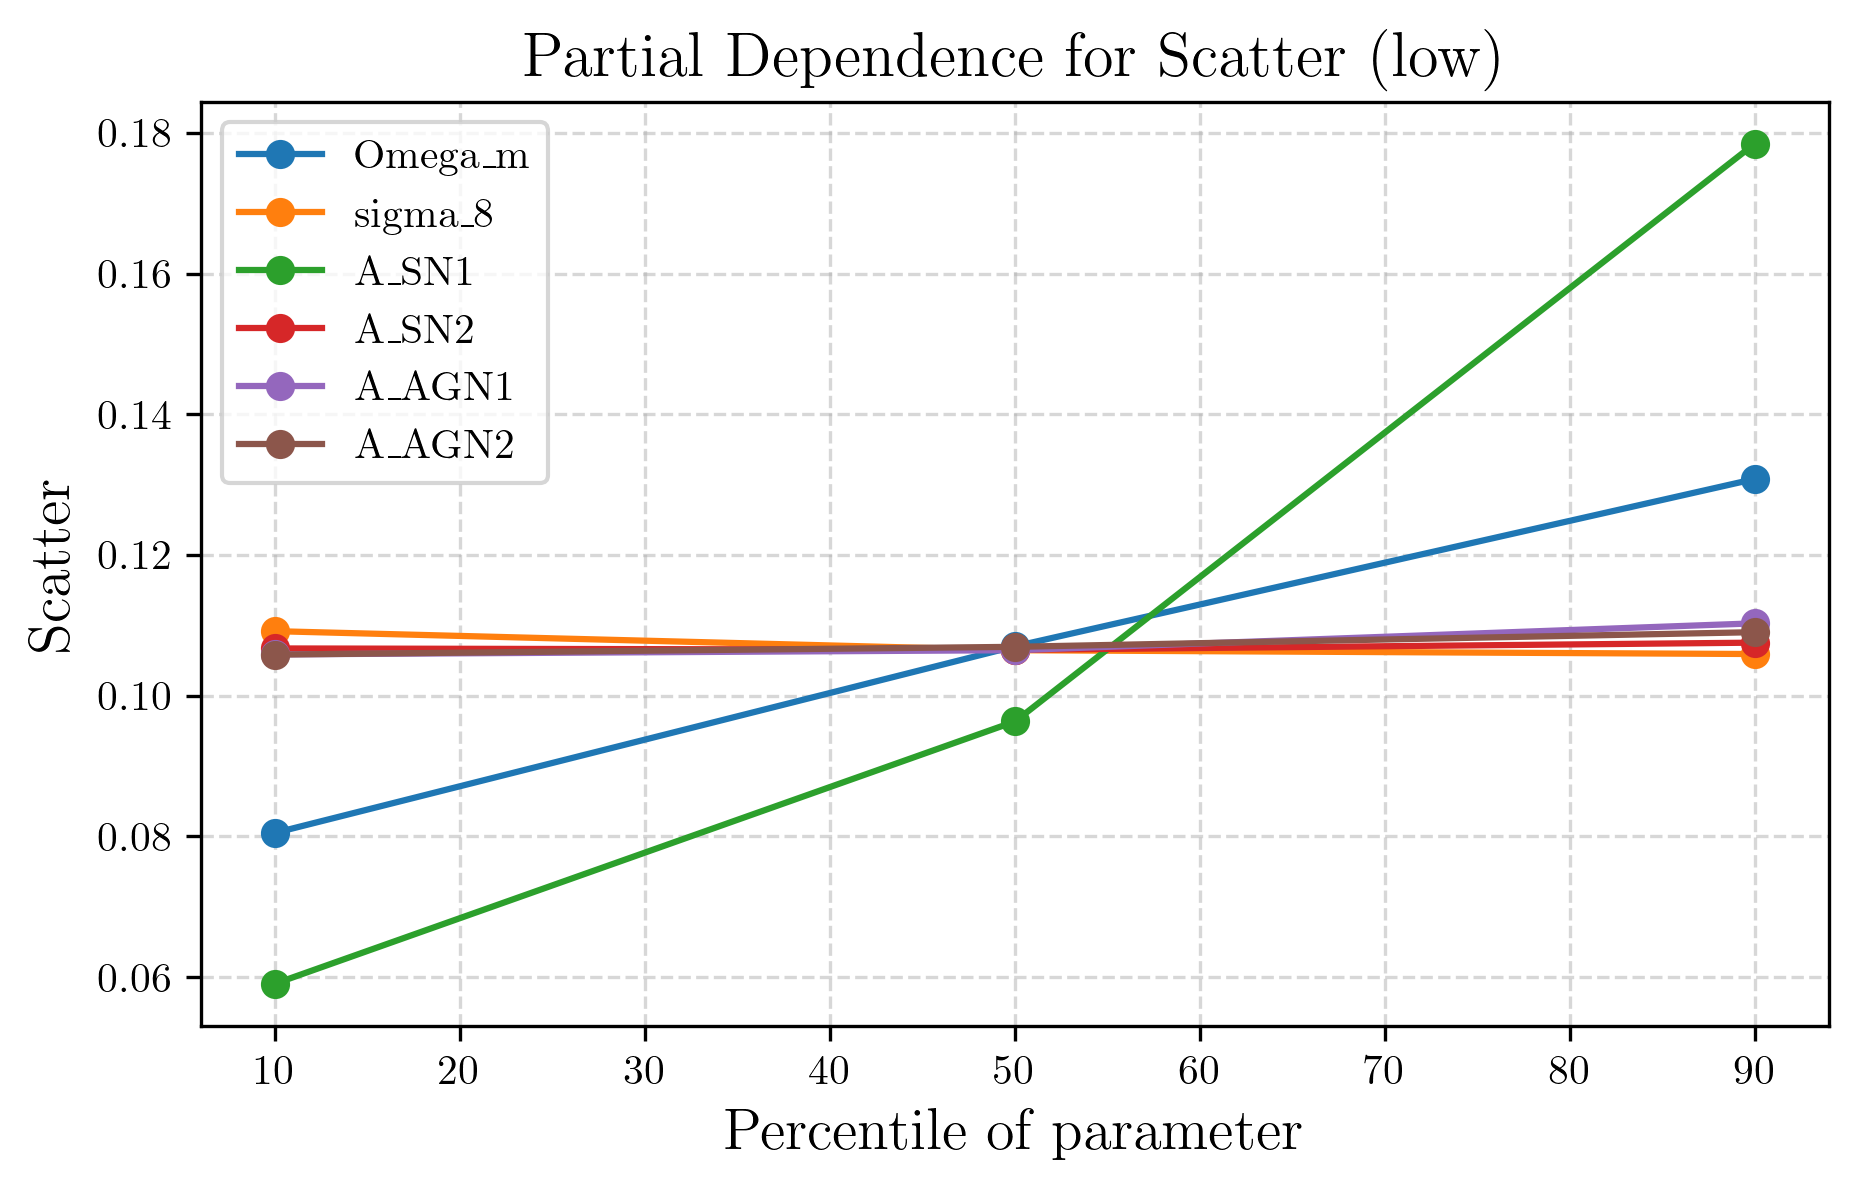
\includegraphics[width=0.5\textwidth]{../Project5/plots/pdp_Scatter_low_35_20250423_182541.png}
    \caption{Partial dependence plot for the scatter in the $M_{\rm BH}$–$M_{\star}$ relation at low stellar mass ($M_{\star}<10^9\,M_\odot$). The scatter is most sensitive to $A_{\rm SN1}$, indicating that stronger SN feedback increases the scatter in black hole masses at a given stellar mass.
}
    \label{fig:pdp_scatter_low}
\end{figure}

\begin{figure}[ht!]
    \centering
    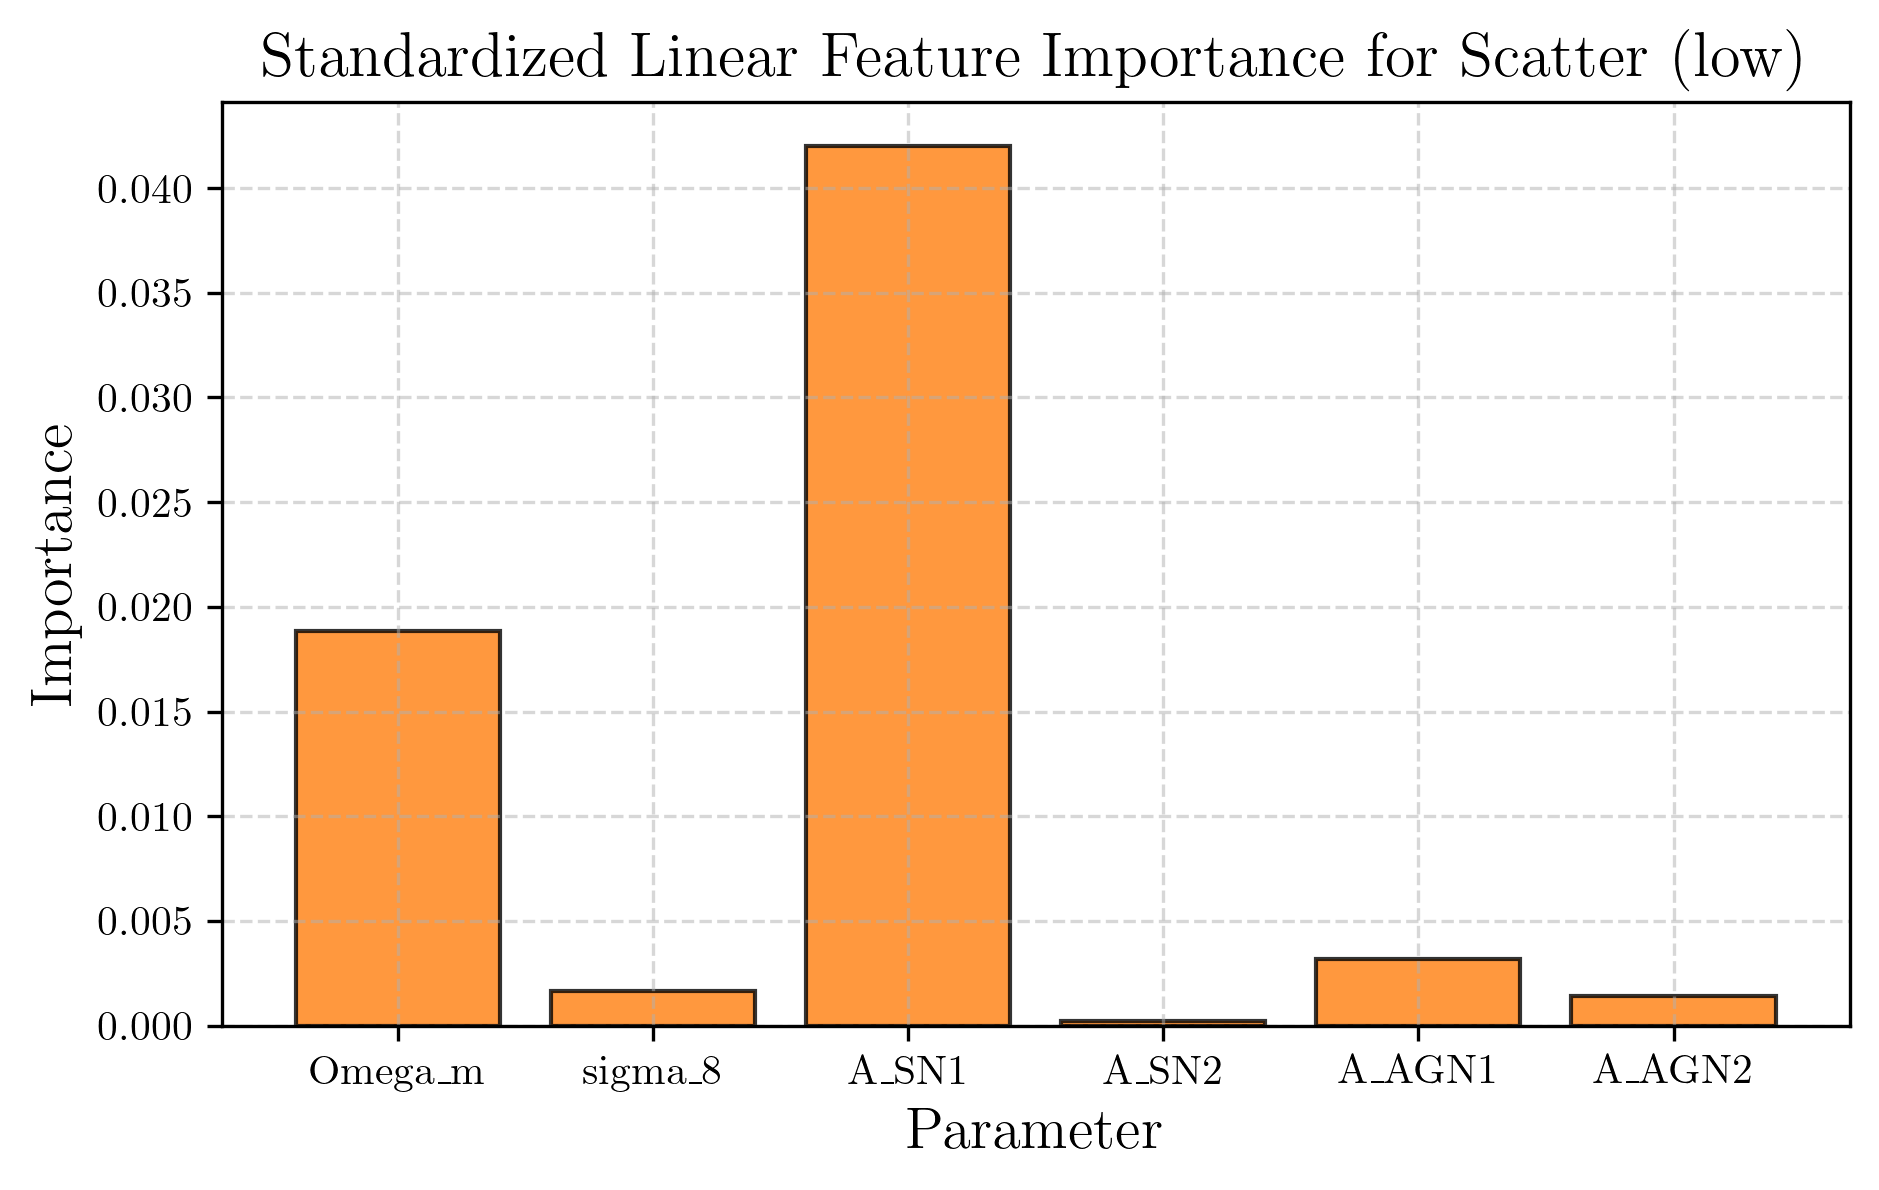
\includegraphics[width=0.5\textwidth]{../Project5/plots/featimp_StandardizedLinear_Scatter_low_34_20250423_182540.png}
    \caption{Standardized linear regression feature importance for the scatter in the $M_{\rm BH}$–$M_{\star}$ relation in the low stellar mass bin. The plot shows that $A_{\rm SN1}$ is the primary driver of increased scatter at low mass, which is consistent with the expectation that stochastic SN feedback introduces diversity in black hole growth histories.
}
    \label{fig:featimp_scatter_low}
\end{figure}

\begin{figure}[ht!]
    \centering
    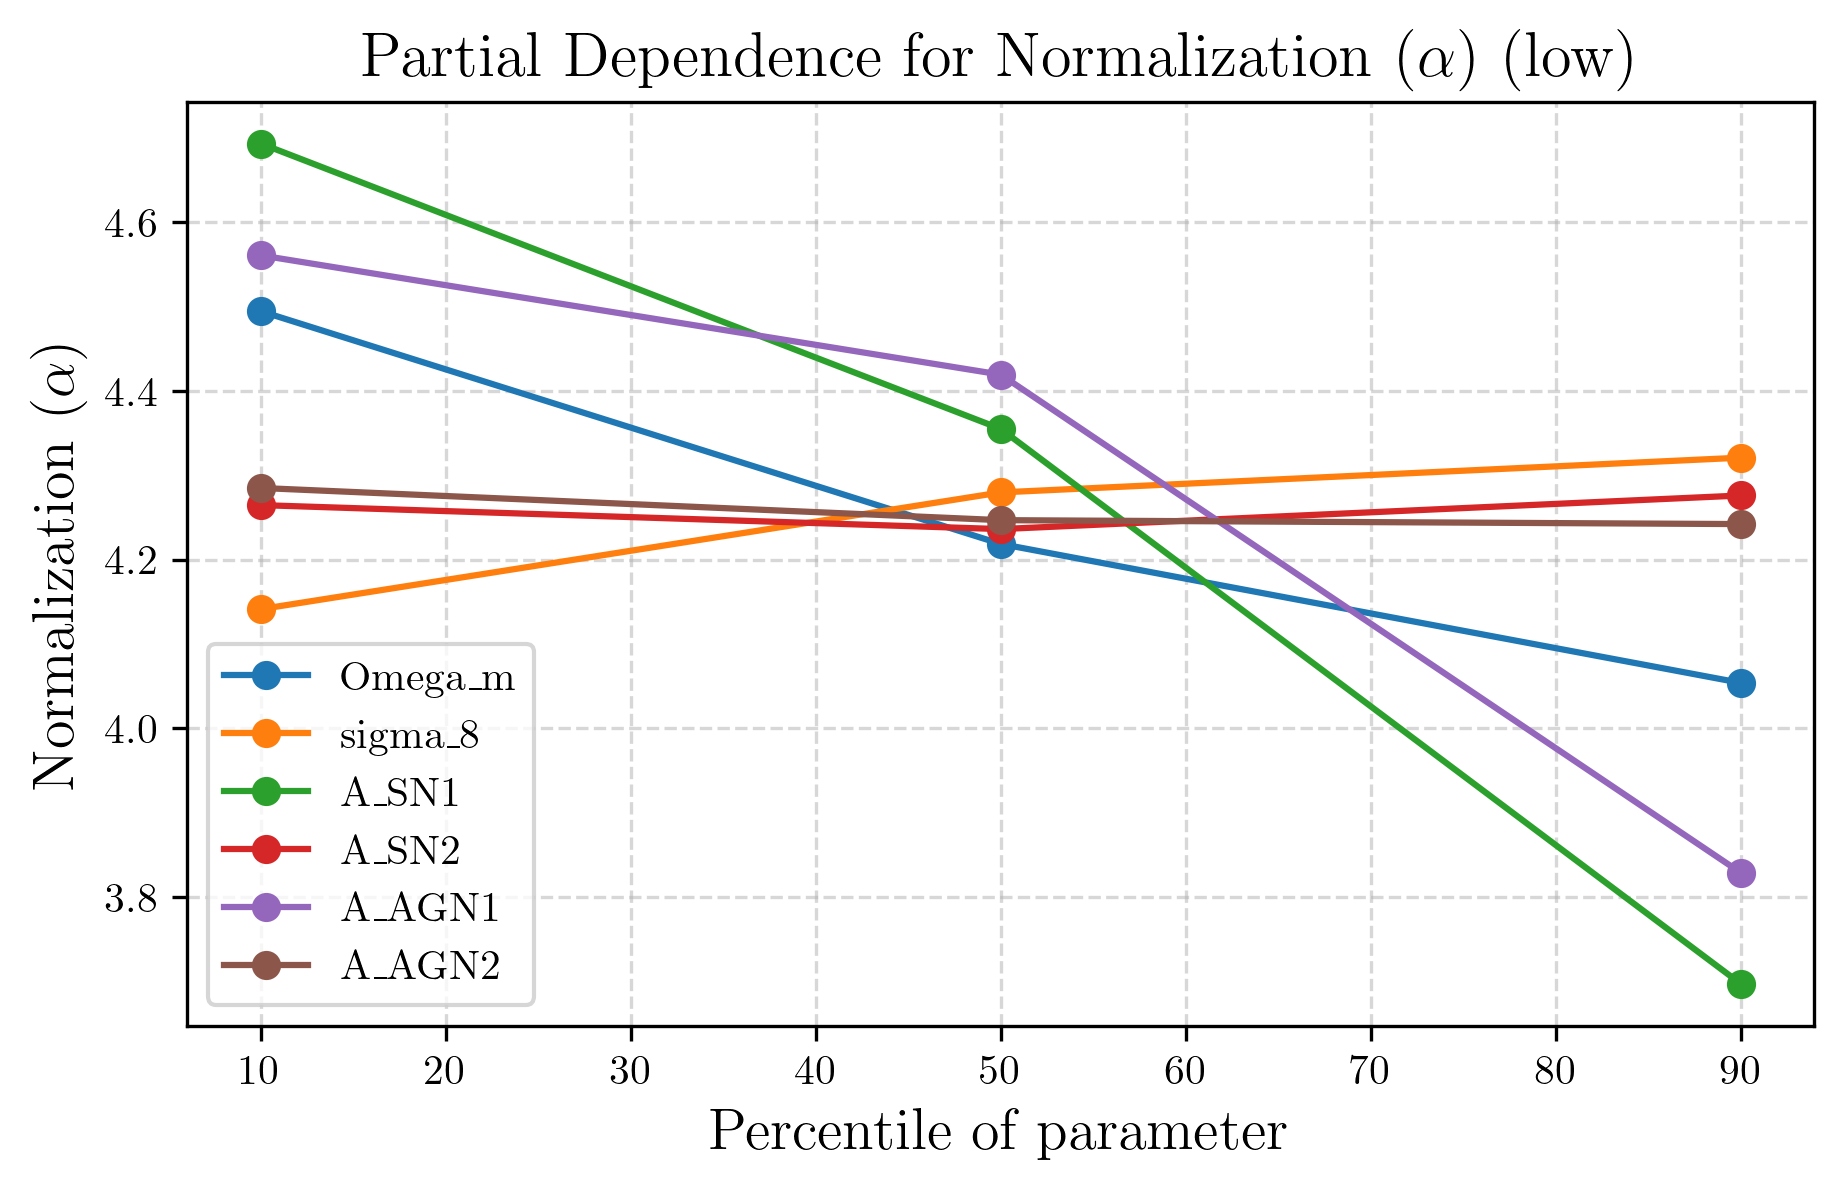
\includegraphics[width=0.5\textwidth]{../Project5/plots/pdp_Normalization_alpha_low_32_20250423_182539.png}
    \caption{Partial dependence plots showing the variation of the black hole-stellar mass relation normalization with cosmological ($\Omega_m$, $\sigma_8$) and feedback ($A_\mathrm{SN1}$, $A_\mathrm{SN2}$, $A_\mathrm{AGN1}$, $A_\mathrm{AGN2}$) parameters in the low stellar mass bin. The normalization is most sensitive to $A_\mathrm{SN1}$ and $A_\mathrm{AGN1}$, indicating that supernova and AGN feedback are the primary drivers of diversity in the black hole-stellar mass relation at low mass.
}
    \label{fig:pdp_norm_low}
\end{figure}

\subsubsection{Intermediate-mass galaxies ($10^9 M_{\odot} \leq M_{\star} < 10^{10} M_{\odot}$)}

In the intermediate-mass bin, the slope ($\beta$) distribution has a mean of 1.06 and a standard deviation of 0.42, ranging from 0.02 to 1.84. The normalization ($\alpha$) has a mean of -3.53 with a standard deviation of 3.80, ranging from -10.6 to 6.05. The intrinsic scatter has a mean of 0.30 dex and a standard deviation of 0.06 dex. The mean black hole occupation fraction is 0.85, with a standard deviation of 0.08.

The slope is closer to unity, indicating a stronger correlation between black hole mass and stellar mass compared to the low-mass bin. The increased scatter suggests that other factors, such as galaxy merger history or AGN feedback, may play a more significant role in determining the black hole mass in this mass range. The higher occupation fraction indicates that most intermediate-mass galaxies host a detectable black hole.

\begin{figure}[ht!]
    \centering
    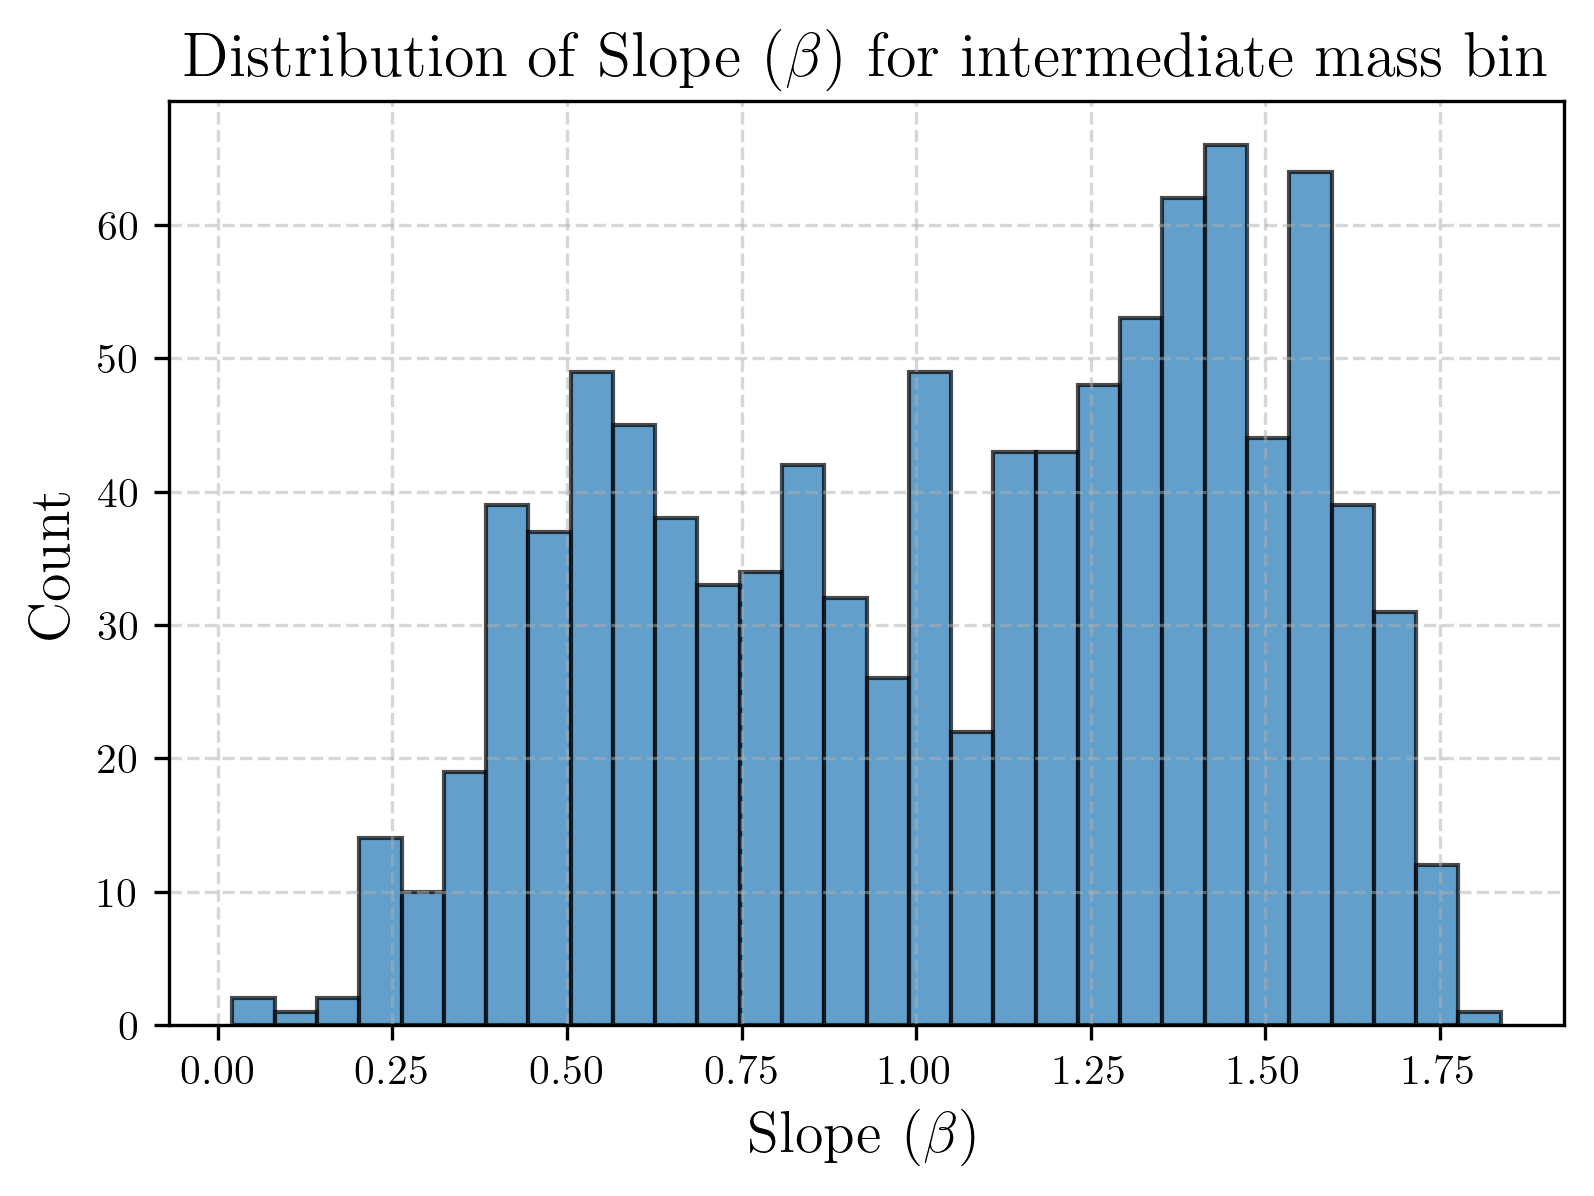
\includegraphics[width=0.5\textwidth]{../Project5/plots/dist_beta_intermediate_42_20250423_182544.png}
    \caption{Histogram of the distribution of slopes ($\beta$) of the $M_\mathrm{BH}$–$M_\mathrm{star}$ relation for the intermediate mass bin ($10^9$–$10^{10}\,M_\odot$) across the 1,000 simulated galaxy catalogs. The diversity in slope highlights the sensitivity of the $M_\mathrm{BH}$–$M_\mathrm{star}$ relation to variations in feedback and cosmological parameters.
}
    \label{fig:dist_beta_intermediate}
\end{figure}

\begin{figure}[ht!]
    \centering
    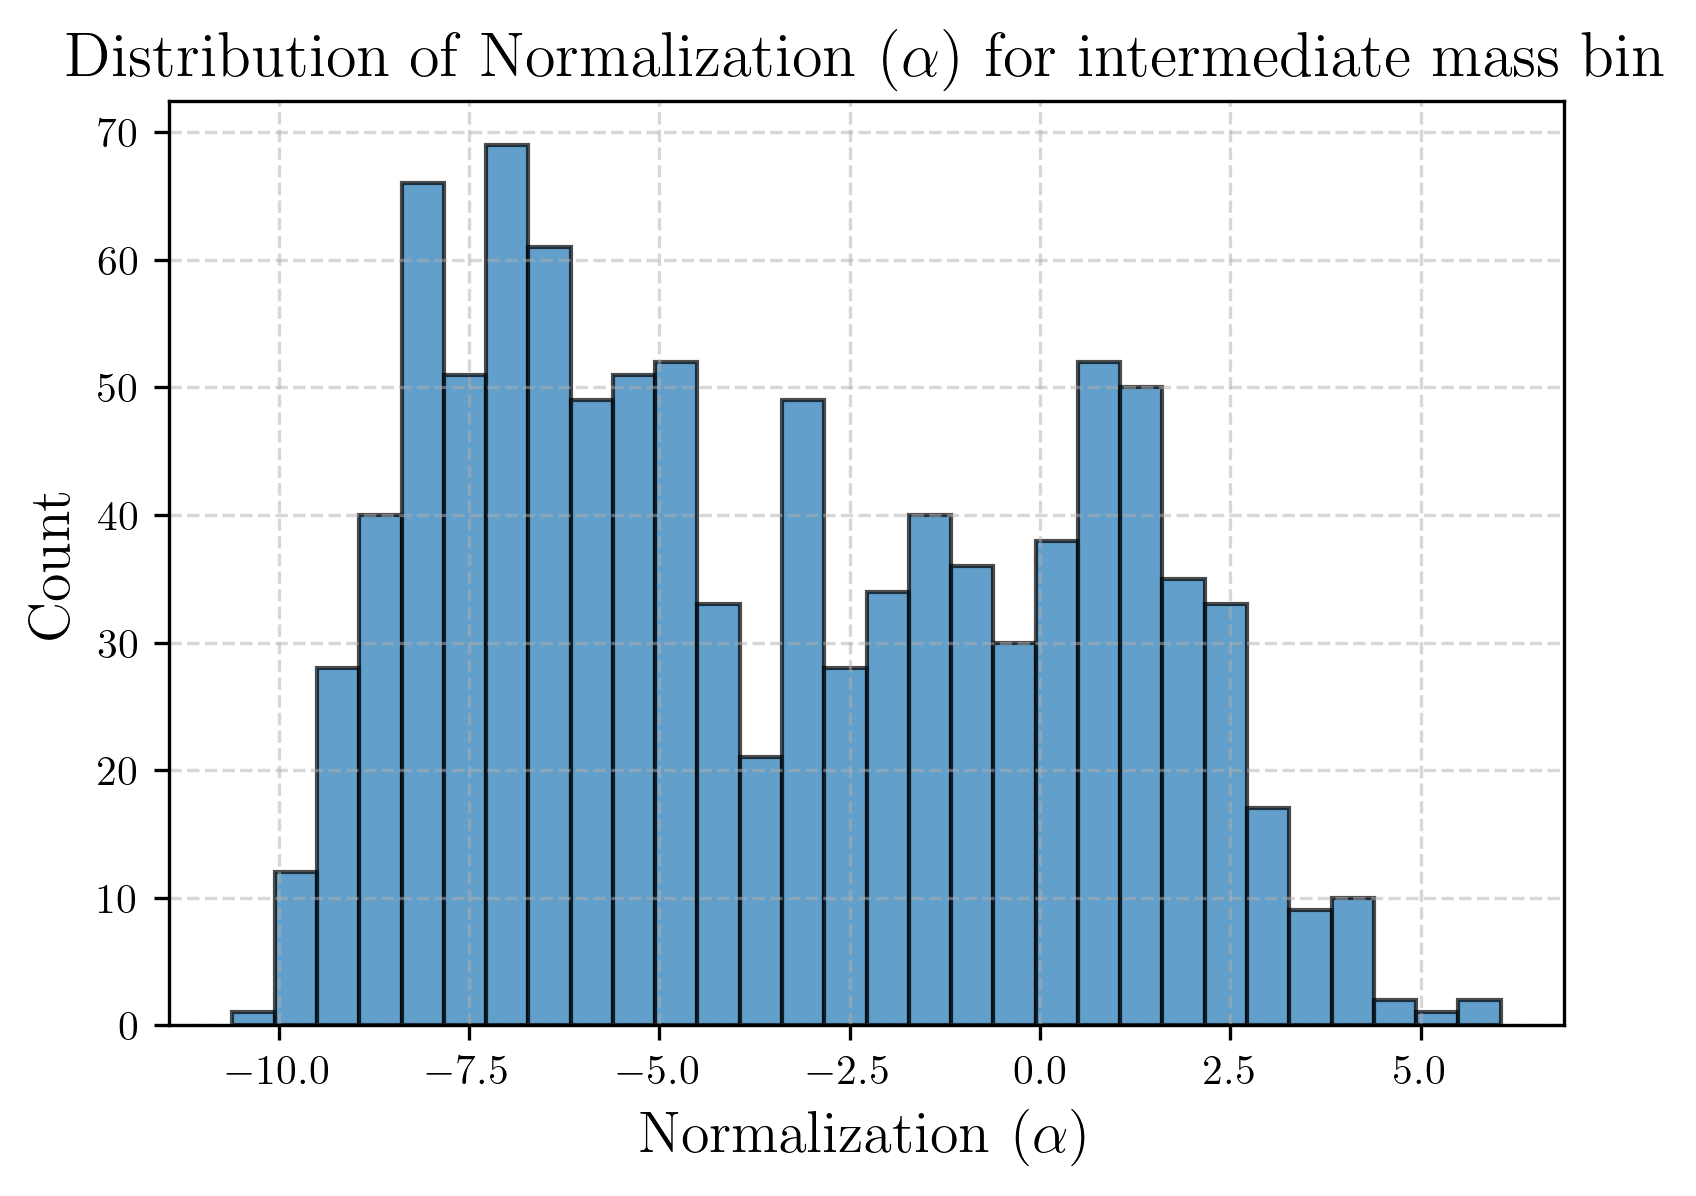
\includegraphics[width=0.5\textwidth]{../Project5/plots/dist_alpha_intermediate_43_20250423_182545.png}
    \caption{Histogram of the normalization ($\alpha$) parameter of the $M_\mathrm{BH}$–$M_\mathrm{star}$ relation for the intermediate mass bin ($10^9$–$10^{10}\,M_\odot$) across the 1,000 simulated galaxy catalogs. The distribution reveals significant diversity in the normalization, indicating a strong sensitivity to feedback and cosmological parameters.
}
    \label{fig:dist_alpha_intermediate}
\end{figure}

\begin{figure}[ht!]
    \centering
    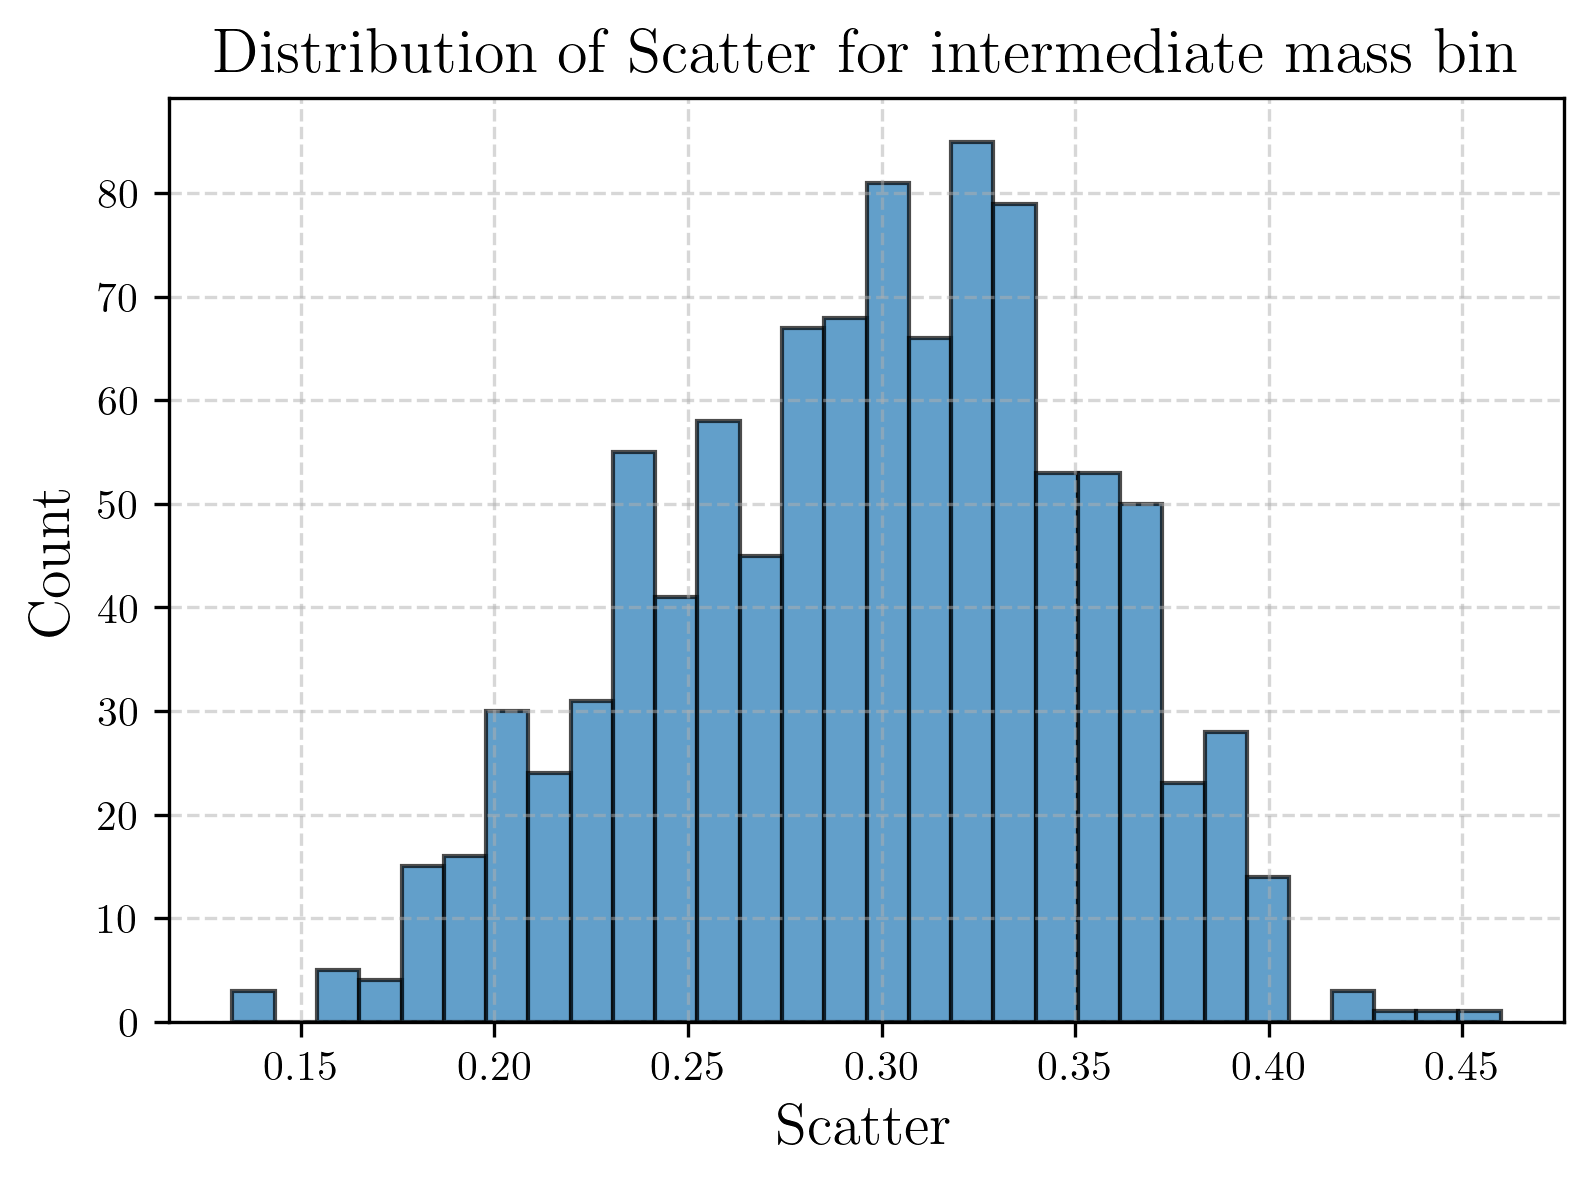
\includegraphics[width=0.5\textwidth]{../Project5/plots/dist_scatter_intermediate_44_20250423_182545.png}
    \caption{Histogram of the intrinsic scatter in the $M_\mathrm{BH}$–$M_\mathrm{star}$ relation for the intermediate mass bin ($10^9-10^{10} M_\odot$) across the 1,000 simulated galaxy catalogs. The scatter varies significantly between simulations, reflecting the diverse effects of feedback and cosmological parameters on black hole and galaxy coevolution.
}
    \label{fig:dist_scatter_intermediate}
\end{figure}

\begin{figure}[ht!]
    \centering
    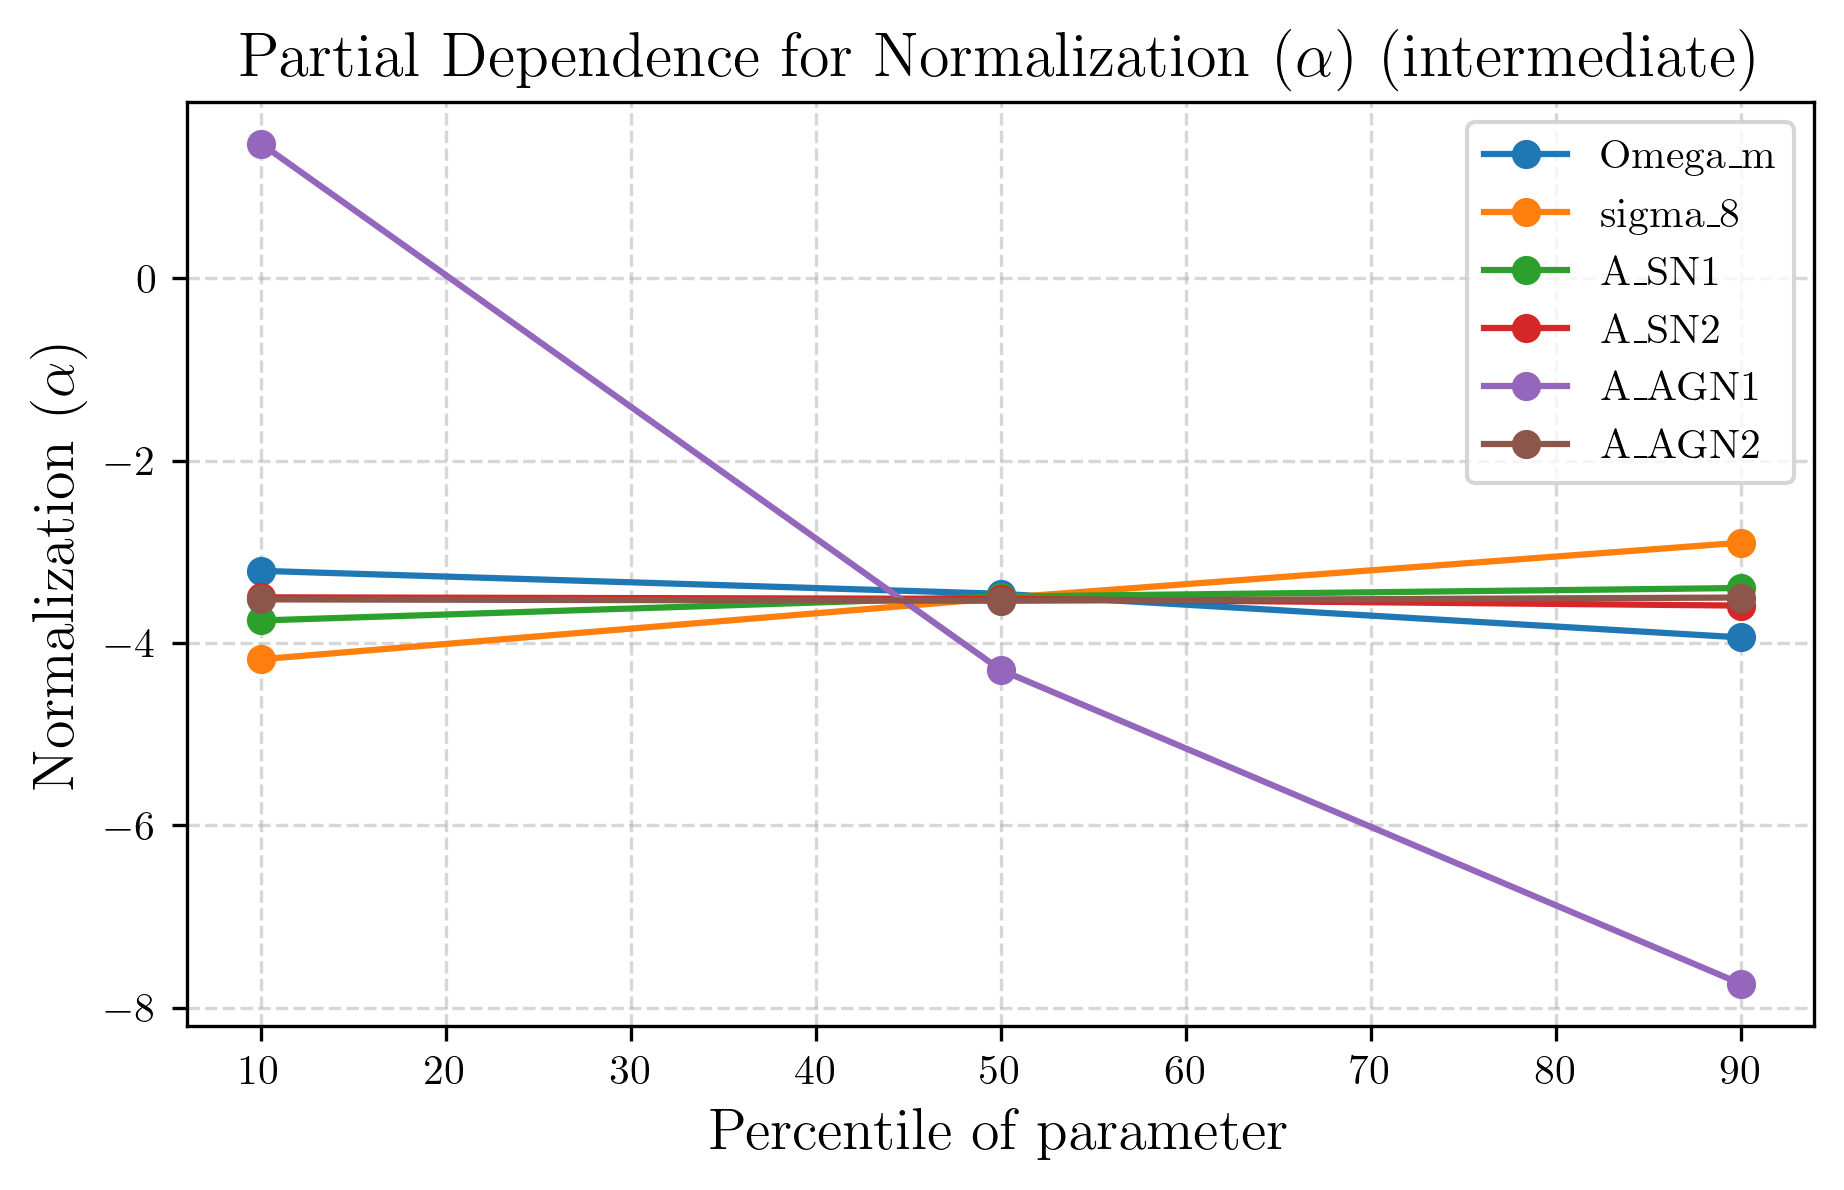
\includegraphics[width=0.5\textwidth]{../Project5/plots/pdp_Normalization_alpha_intermediate_74_20250423_182559.png}
    \caption{Partial dependence plot showing the influence of cosmological and feedback parameters on the normalization of the $M_{\rm BH}$–$M_{\star}$ relation in the intermediate mass bin. Strong AGN feedback (A\ensuremath{\_}AGN1) significantly decreases the normalization, while other parameters have weaker effects.
}
    \label{fig:pdp_norm_intermediate}
\end{figure}

\begin{figure}[ht!]
    \centering
    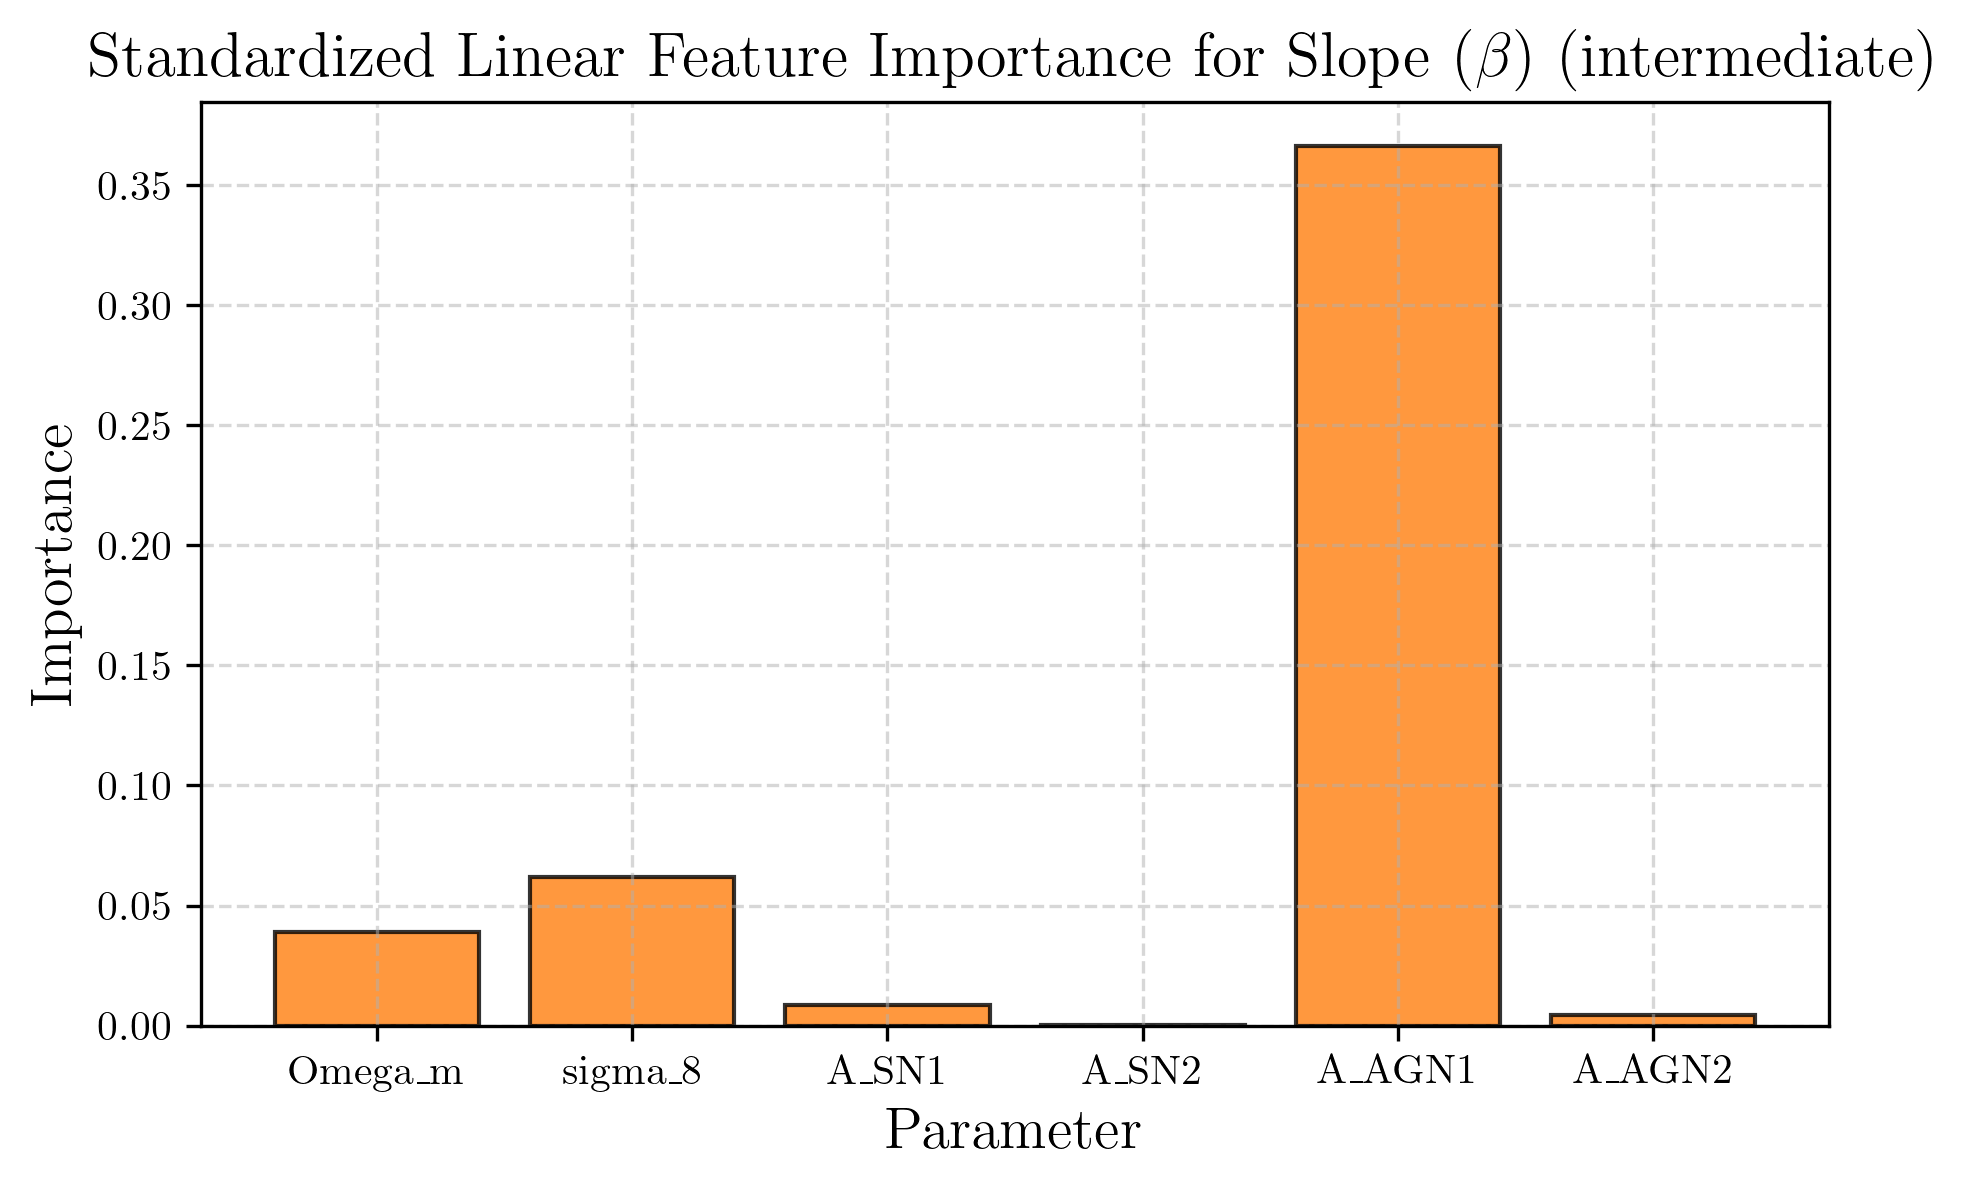
\includegraphics[width=0.5\textwidth]{../Project5/plots/featimp_StandardizedLinear_Slope_beta_intermediate_70_20250423_182558.png}
    \caption{Standardized linear regression feature importance for the slope of the $M_\mathrm{BH}$–$M_\mathrm{star}$ relation in the intermediate mass bin. The AGN feedback parameter ($A_\mathrm{AGN1}$) is the dominant factor influencing the slope.
}
    \label{fig:featimp_slope_linear_intermediate}
\end{figure}

\begin{figure}[ht!]
    \centering
    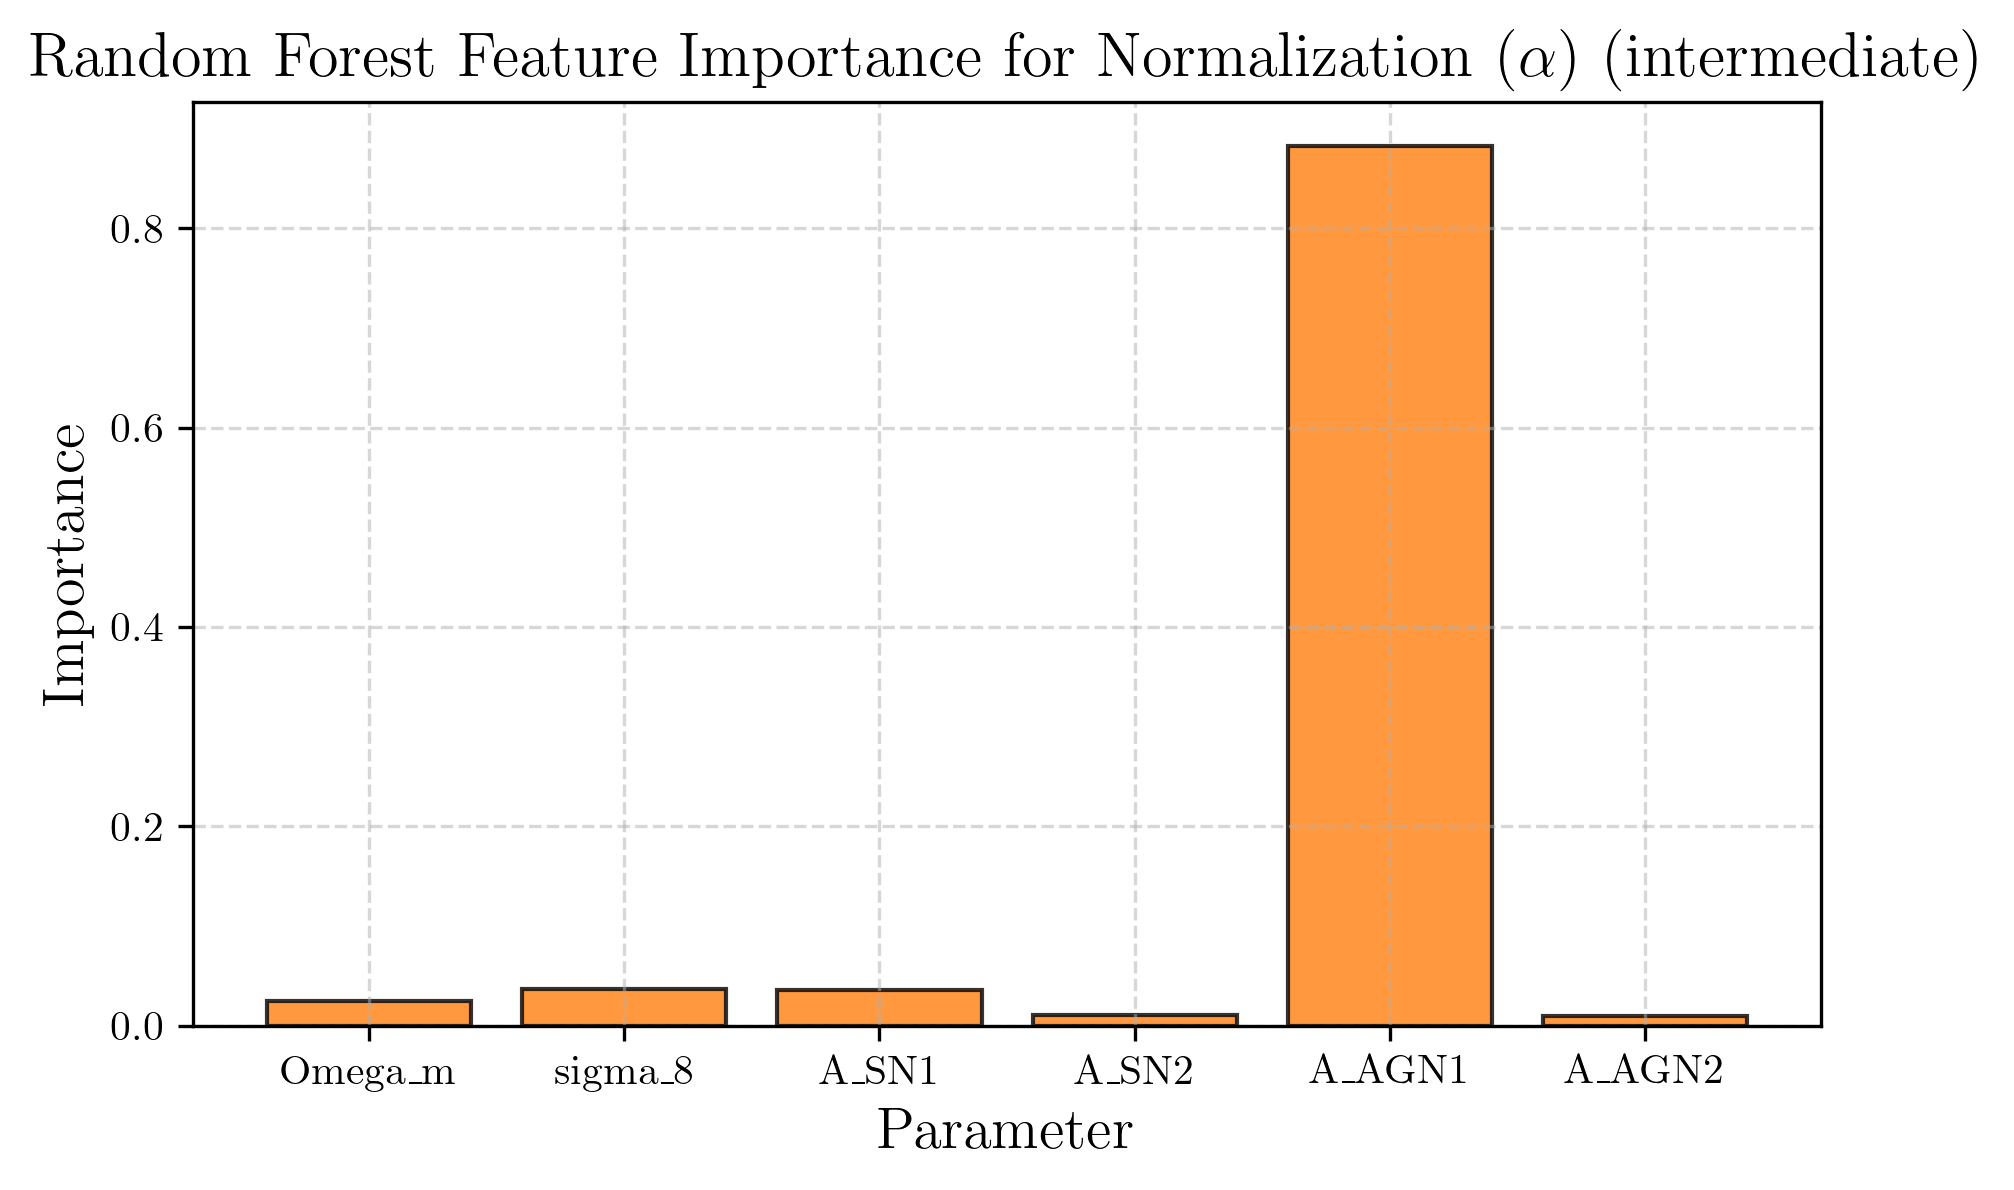
\includegraphics[width=0.5\textwidth]{../Project5/plots/featimp_RandomForest_Normalization_alpha_intermediate_72_20250423_182559.png}
    \caption{Random forest feature importance for the normalization of the $M_\mathrm{BH}$–$M_\mathrm{star}$ relation in the intermediate mass bin. The $A_\mathrm{AGN1}$ parameter dominates the normalization, indicating that AGN feedback is the primary driver in this mass range.
}
    \label{fig:featimp_norm_random_intermediate}
\end{figure}

\subsubsection{High-mass galaxies ($M_{\star} \geq 10^{10} M_{\odot}$)}

For high-mass galaxies, the slope ($\beta$) has a mean of 1.22 and a standard deviation of 0.30, ranging from 0.03 to 2.07. The normalization ($\alpha$) has a mean of -4.85 with a standard deviation of 3.39, ranging from -14.2 to 7.64. The intrinsic scatter has a mean of 0.40 dex and a standard deviation of 0.14 dex. The mean black hole occupation fraction is 0.96, with a standard deviation of 0.03.

The slope is close to unity, consistent with the canonical $M_{\rm BH}$--$M_{\star}$ relation. The large scatter suggests that the relationship between black hole mass and stellar mass is more complex in these massive galaxies, potentially due to AGN feedback or galaxy mergers. The occupation fraction is close to unity, indicating that nearly all high-mass galaxies host a detectable black hole.

\begin{figure}[ht!]
    \centering
    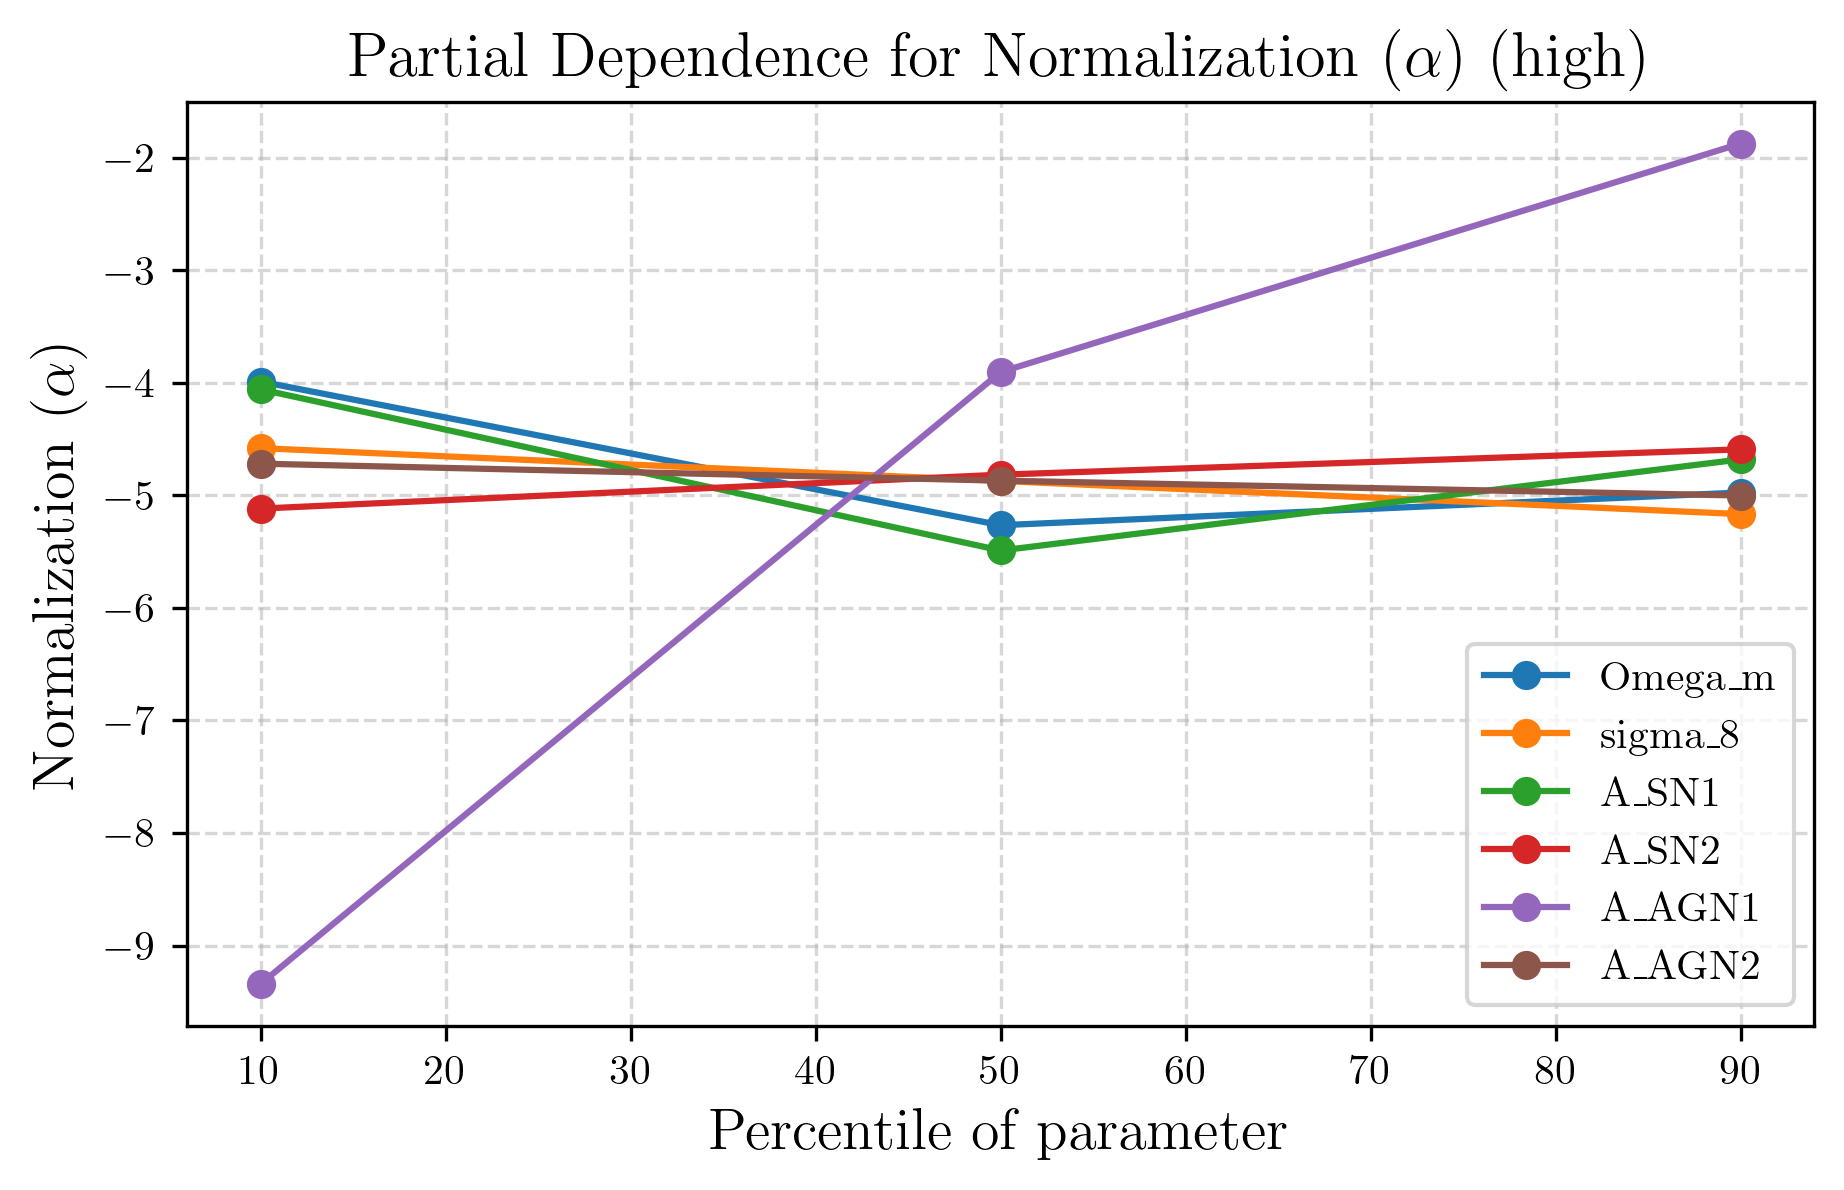
\includegraphics[width=0.5\textwidth]{../Project5/plots/pdp_Normalization_alpha_high_116_20250423_182620.png}
    \caption{Partial dependence plots showing the influence of cosmological and feedback parameters on the normalization of the $M_\mathrm{BH}$–$M_\mathrm{star}$ relation for galaxies in the high mass bin ($M_\mathrm{star} > 10^{10} M_\odot$). The normalization exhibits a strong dependence on $A_\mathrm{AGN1}$, and weaker dependencies on other parameters, indicating that AGN feedback is a key driver of the relation's normalization at high mass.
}
    \label{fig:pdp_norm_high}
\end{figure}

\begin{figure}[ht!]
    \centering
    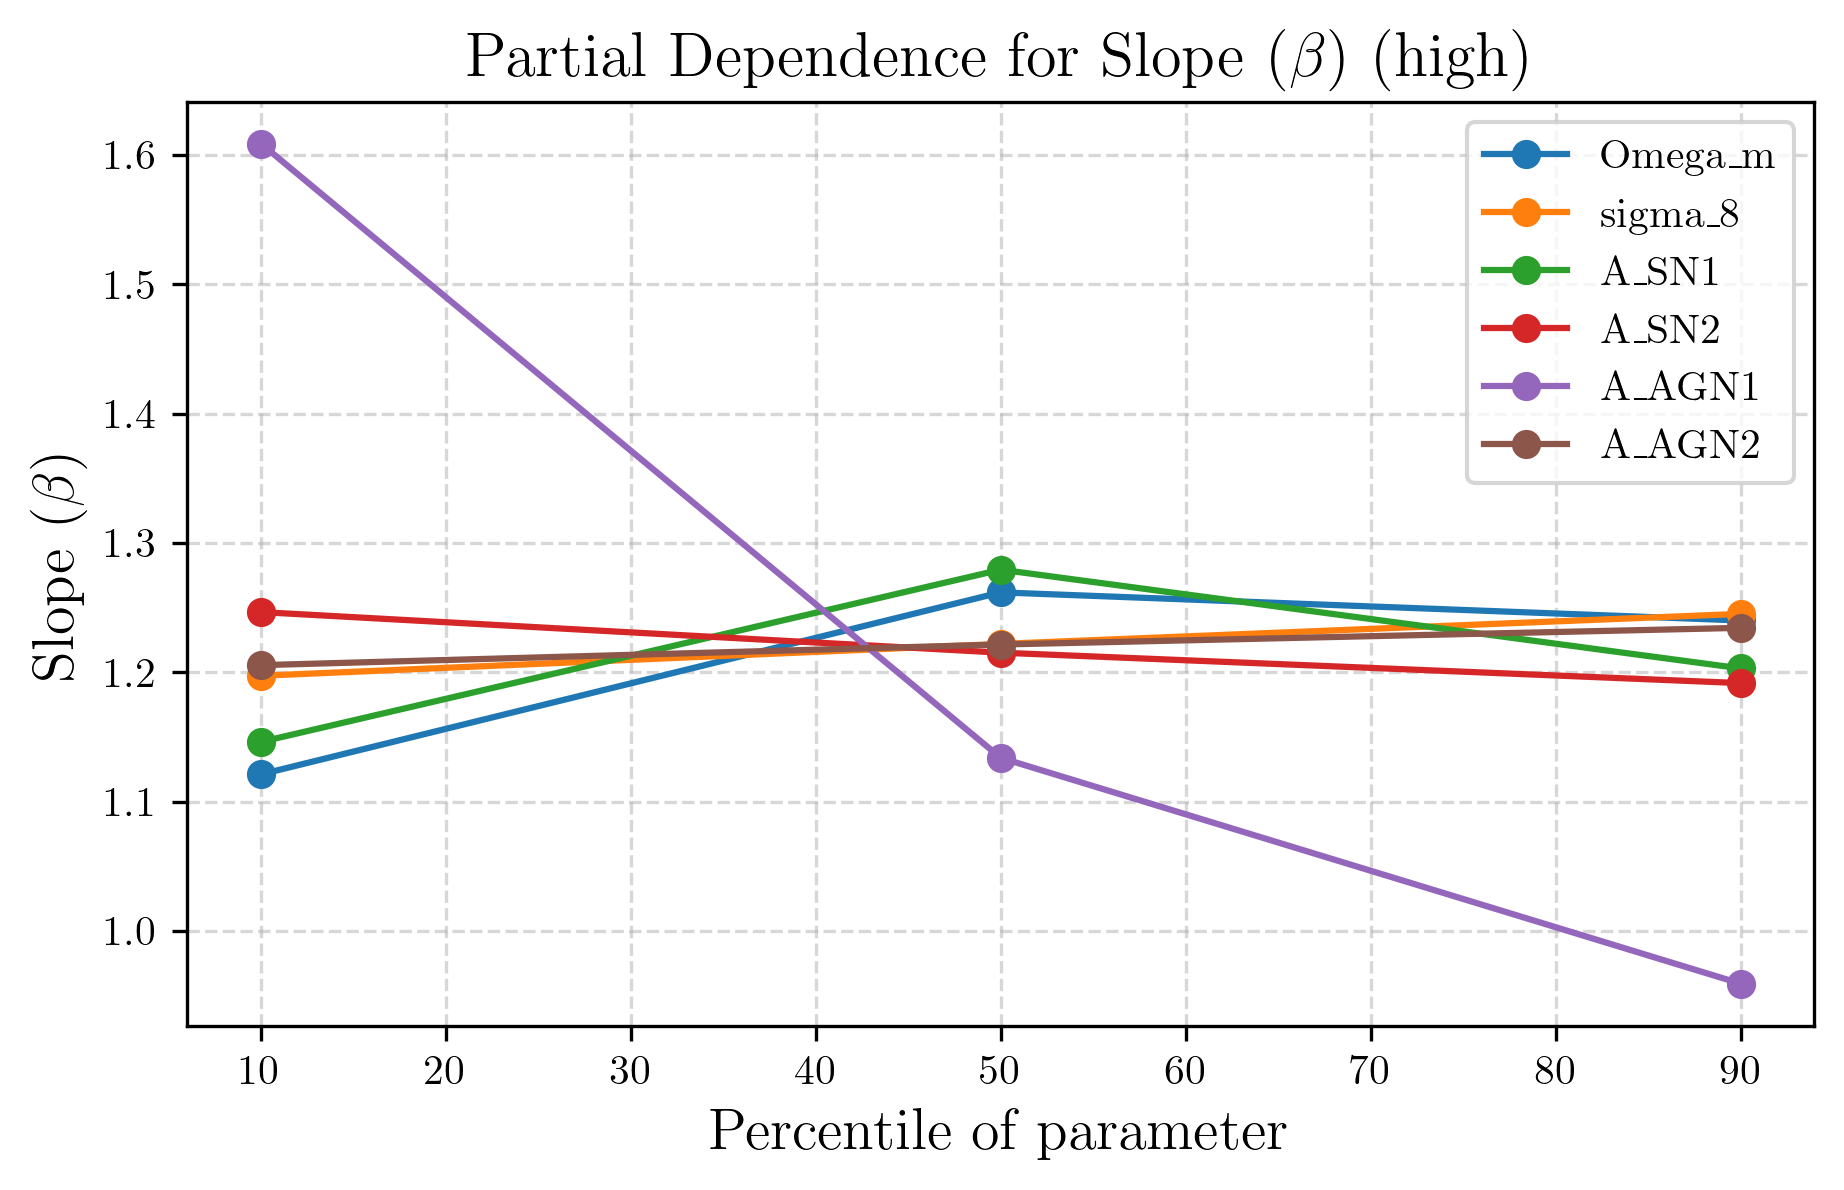
\includegraphics[width=0.5\textwidth]{../Project5/plots/pdp_Slope_beta_high_113_20250423_182618.png}
    \caption{Partial dependence plots showing the variation of the $M_\mathrm{BH}$–$M_\mathrm{star}$ relation slope ($\beta$) in the high mass bin as a function of cosmological ($\Omega_m$) and feedback ($A_\mathrm{SN1}$, $A_\mathrm{SN2}$, $A_\mathrm{AGN1}$, $A_\mathrm{AGN2}$) parameters. The slope exhibits a strong dependence on $A_\mathrm{AGN1}$, suggesting a key role for AGN feedback in regulating the $M_\mathrm{BH}$–$M_\mathrm{star}$ relation at high stellar masses.
}
    \label{fig:pdp_slope_high}
\end{figure}

\begin{figure}[ht!]
    \centering
    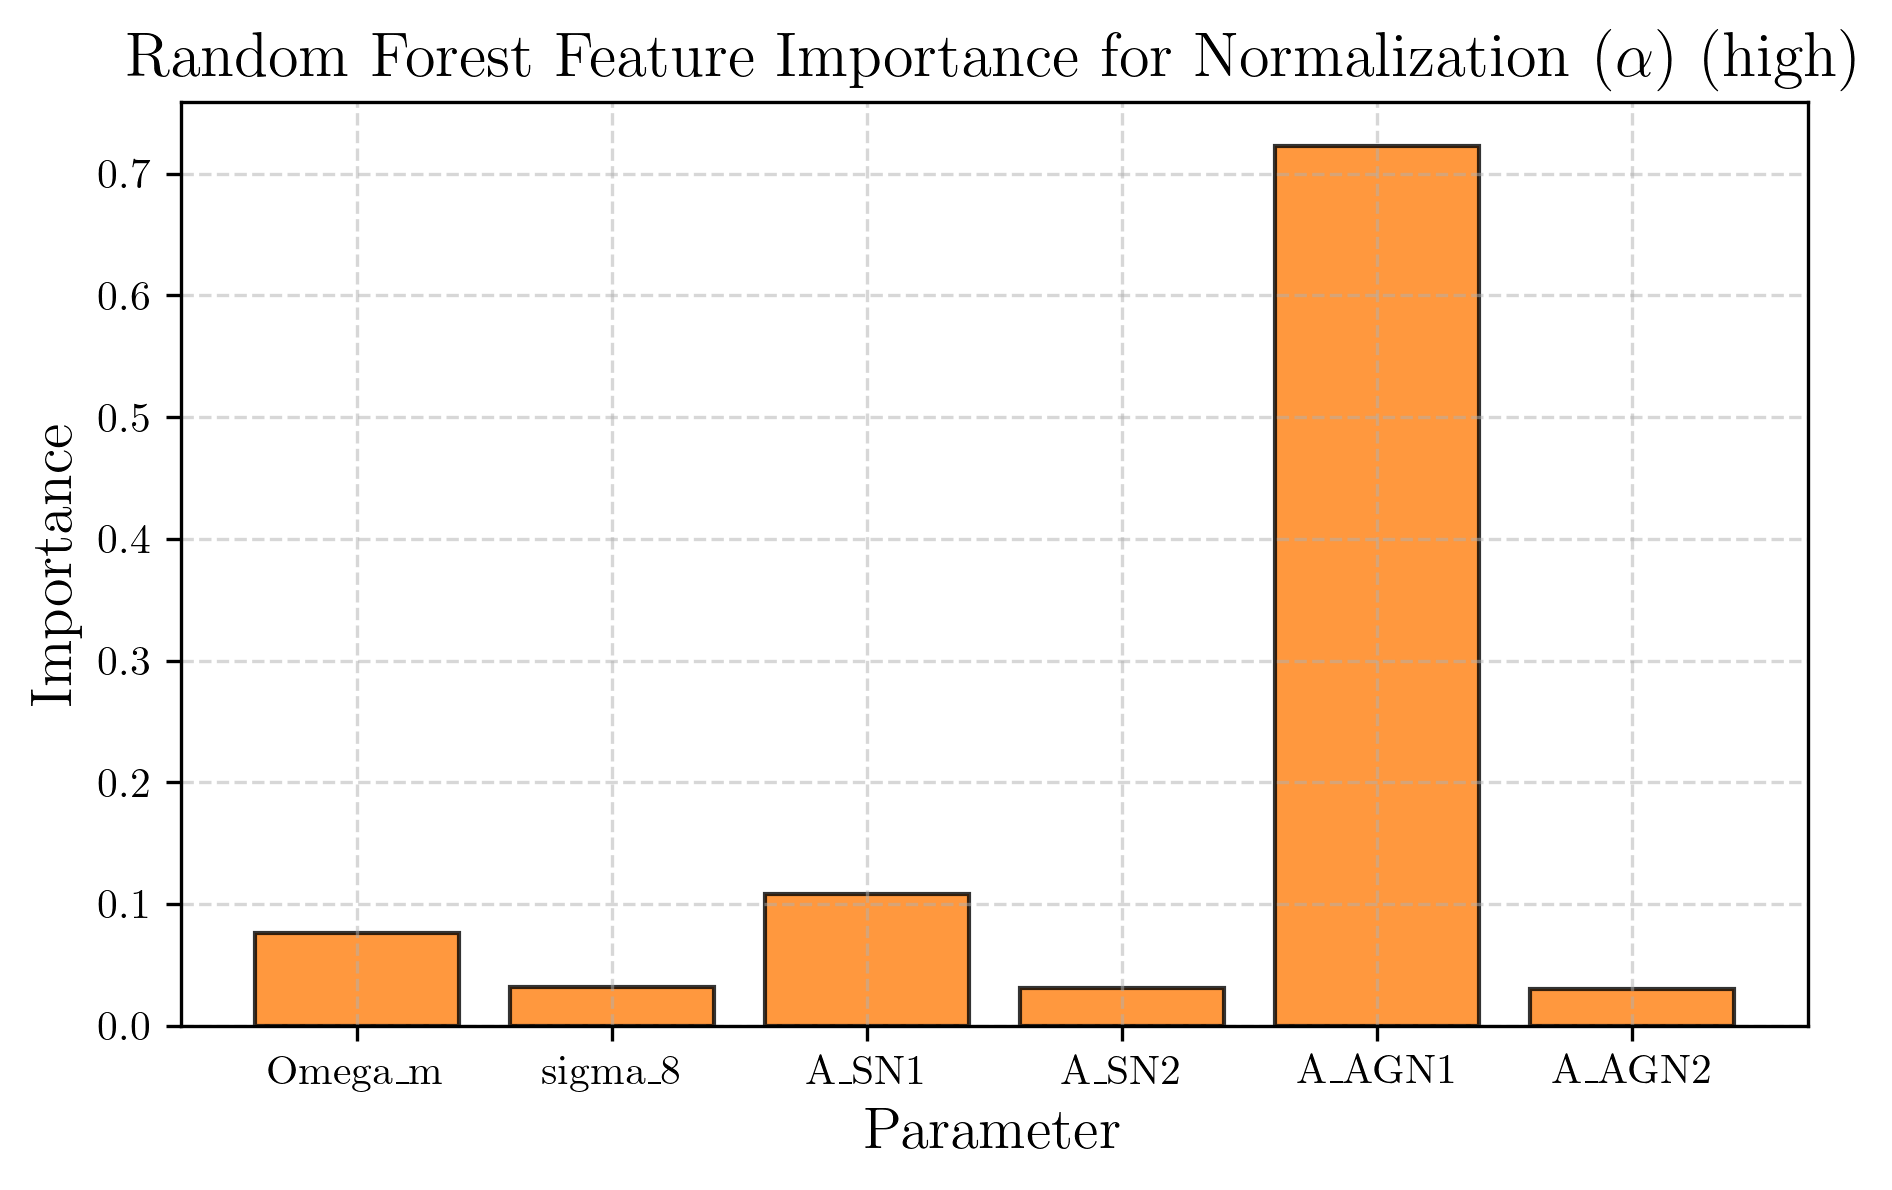
\includegraphics[width=0.5\textwidth]{../Project5/plots/featimp_RandomForest_Normalization_alpha_high_114_20250423_182619.png}
    \caption{Random forest feature importance for the normalization of the $M_{\rm BH}$–$M_{\star}$ relation in the high mass bin ($M_{\star} > 10^{10} M_\odot$). The AGN feedback energy per accretion ($A_{\rm AGN1}$) is the dominant parameter.
}
    \label{fig:featimp_norm_high}
\end{figure}

\begin{figure}[ht!]
    \centering
    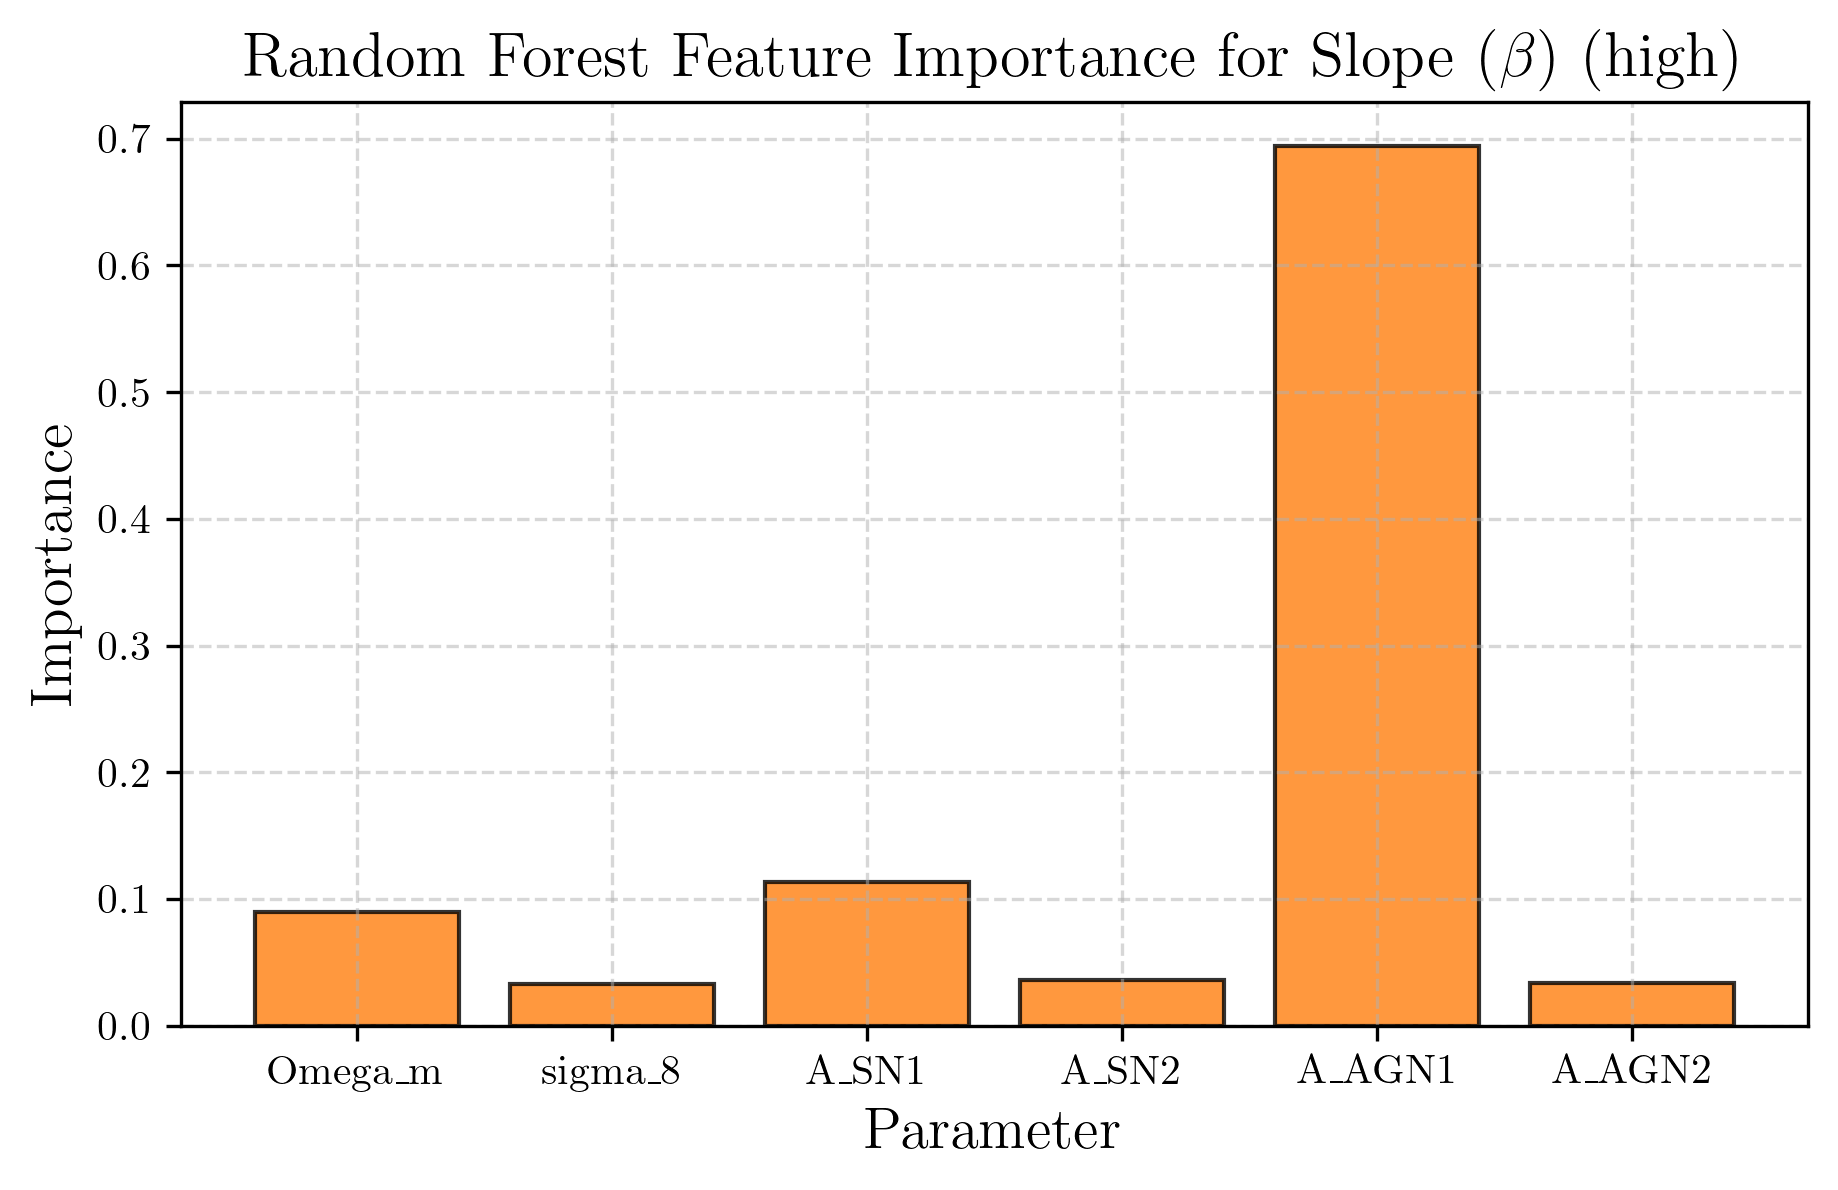
\includegraphics[width=0.5\textwidth]{../Project5/plots/featimp_RandomForest_Slope_beta_high_111_20250423_182617.png}
    \caption{Random forest feature importance for the slope of the black hole - stellar mass relation in the high mass bin ($M_\mathrm{star}>10^{10}\,M_\odot$). The AGN feedback parameter $A_\mathrm{AGN1}$ is the dominant factor, indicating that AGN feedback plays a crucial role in shaping the $M_\mathrm{BH}$–$M_\mathrm{star}$ relation in massive galaxies.
}
    \label{fig:featimp_slope_random_high}
\end{figure}

\begin{figure}[ht!]
    \centering
    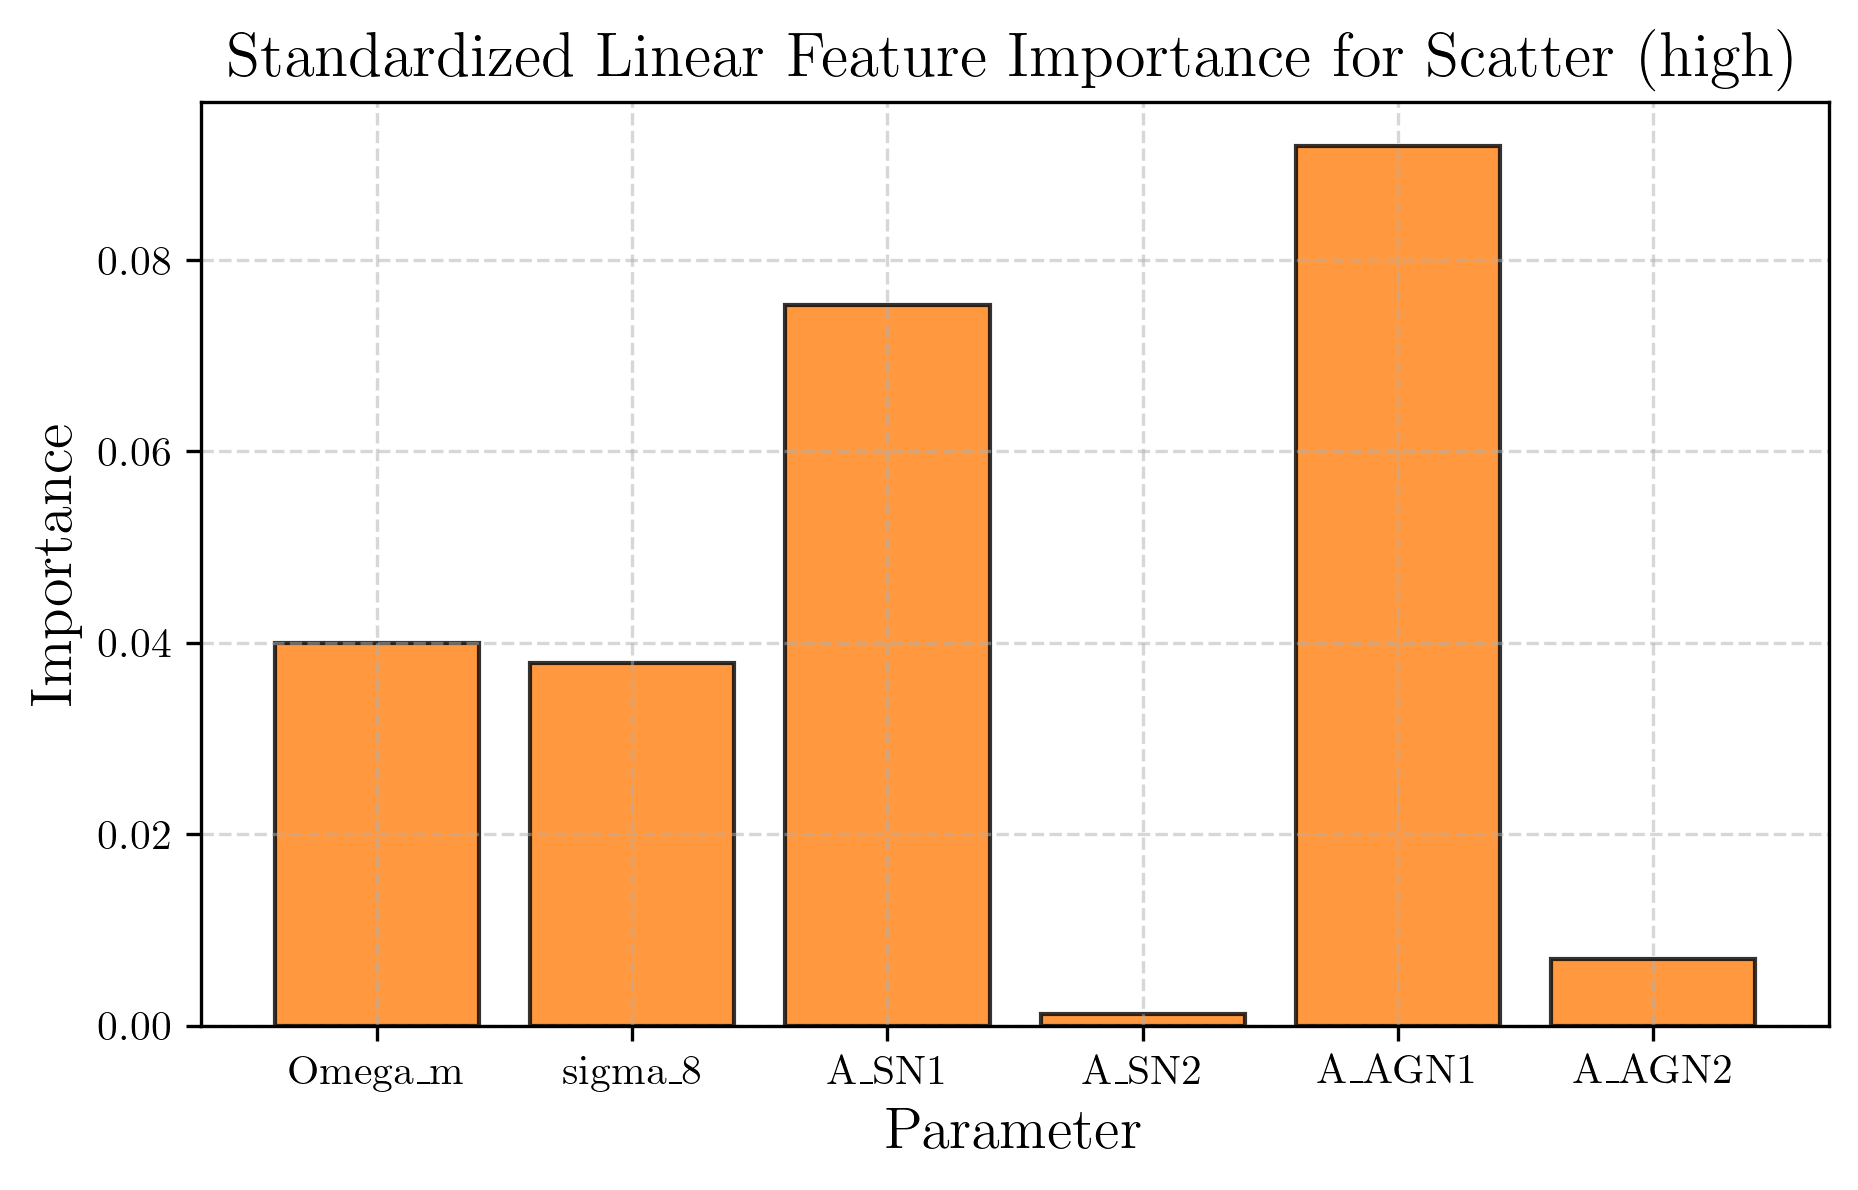
\includegraphics[width=0.5\textwidth]{../Project5/plots/featimp_StandardizedLinear_Scatter_high_118_20250423_182621.png}
    \caption{Standardized linear regression feature importance for the scatter in the $M_\mathrm{BH}$–$M_\mathrm{star}$ relation at high stellar mass ($>10^{10}\,M_\odot$). The scatter is most sensitive to $A_\mathrm{AGN1}$ and $A_\mathrm{SN1}$, suggesting that both AGN and supernova feedback introduce diversity in black hole growth histories.
}
    \label{fig:featimp_scatter_linear_high}
\end{figure}

\subsection{Dependence on Feedback and Cosmological Parameters}

To quantify the influence of feedback and cosmological parameters on the $M_{\rm BH}$--$M_{\star}$ relation, we performed multivariate regression analysis.

\subsubsection{Low-mass galaxies}

In the low-mass regime, the slope ($\beta$) is most influenced by the supernova feedback parameter A\ensuremath{\_}{SN1} and AGN feedback parameter A\ensuremath{\_}{AGN1}. The standardized coefficient for A\ensuremath{\_}{SN1} is +0.05, and its random forest feature importance is 0.41. For A\ensuremath{\_}{AGN1}, the standardized coefficient is +0.04, and its random forest feature importance is 0.29. Both parameters positively correlate with the slope, suggesting that stronger feedback steepens the relation in low-mass galaxies. The normalization ($\alpha$) is strongly negatively correlated with A\ensuremath{\_}{SN1} (coefficient -0.38) and A\ensuremath{\_}{AGN1} (coefficient -0.32), indicating that stronger feedback leads to lower black hole masses at a fixed stellar mass. The intrinsic scatter is primarily driven by A\ensuremath{\_}{SN1} (coefficient +0.04, random forest importance 0.73), consistent with the expectation that stochastic supernova feedback introduces diversity in black hole growth histories.

\subsubsection{Intermediate-mass galaxies}

In the intermediate-mass regime, the slope ($\beta$) is dominated by the AGN feedback parameter A\ensuremath{\_}{AGN1} (coefficient +0.37, random forest importance 0.88). This suggests that AGN feedback plays a significant role in regulating black hole growth in intermediate-mass galaxies. The normalization ($\alpha$) is also strongly influenced by A\ensuremath{\_}{AGN1} (coefficient -3.32). The intrinsic scatter is influenced by both A\ensuremath{\_}{AGN1} and A\ensuremath{\_}{SN1}.

\subsubsection{High-mass galaxies}

In high-mass galaxies, the slope ($\beta$) is dominated by the AGN feedback parameter A\ensuremath{\_}{AGN1} (coefficient -0.22, random forest importance 0.69), but the sign of the coefficient is reversed compared to the intermediate-mass bin, indicating a shift in the role of AGN feedback. The normalization ($\alpha$) is also strongly influenced by A\ensuremath{\_}{AGN1} (coefficient +2.52). The intrinsic scatter is influenced by both A\ensuremath{\_}{AGN1} and A\ensuremath{\_}{SN1}.

\subsection{Black Hole Occupation Fraction}

The black hole occupation fraction increases with stellar mass, rising from approximately 0.72 in low-mass galaxies to nearly 0.96 in high-mass galaxies. The occupation fraction also depends on feedback parameters, with stronger supernova feedback (A\ensuremath{\_}{SN1}) reducing the occupation fraction at low and intermediate masses, consistent with the suppression of black hole formation or growth in shallow potential wells.

\subsection{Synthesis}

The results demonstrate that the diversity in the $M_{\rm BH}$--$M_{\star}$ relation is primarily driven by the strength and mode of feedback, with supernova feedback dominating at low mass and AGN feedback at high mass. Cosmological parameters also modulate the normalization and scatter, particularly in the intermediate and high mass bins. The black hole occupation fraction increases with stellar mass and is suppressed by supernova feedback at low mass. These findings highlight the importance of feedback physics in shaping the coevolution of black holes and galaxies, and provide a framework for interpreting the observed diversity in black hole scaling relations.

In summary, we find that supernova feedback plays a dominant role in regulating the $M_{\rm BH}$--$M_{\star}$ relation and black hole occupation fraction in low-mass galaxies, while AGN feedback becomes increasingly important in intermediate and high-mass galaxies. Cosmological parameters have a secondary but non-negligible influence on the normalization and scatter of the relation. These results emphasize the complex interplay of various physical processes in shaping the coevolution of black holes and galaxies.

\section{Conclusions}
\label{sec:conclusions}
This study addresses the open question of the universality of the black hole-stellar mass ($M_{\rm BH}$--$M_{\star}$) relation, a cornerstone of galaxy evolution. We systematically quantify how the slope, normalization, and scatter of this relation change in response to variations in cosmological parameters and feedback processes.

Using a suite of simulated galaxies, each representing a unique combination of cosmological and feedback parameters, we fit the $M_{\rm BH}$--$M_{\star}$ relation within different stellar mass ranges, focusing on galaxies hosting black holes. We employ multivariate regression and random forest analysis to map how the relation's parameters depend on the input cosmological and feedback parameters.

Our results demonstrate that feedback, particularly from supernovae in low-mass galaxies and active galactic nuclei in high-mass galaxies, is the dominant factor driving diversity in the $M_{\rm BH}$--$M_{\star}$ relation. Cosmological parameters influence the normalization and scatter, while the fraction of galaxies hosting black holes is sensitive to feedback, especially in low-mass systems. Specifically, in low-mass galaxies ($M_{\star} < 10^9 M_{\odot}$), the slope of the $M_{\rm BH}$--$M_{\star}$ relation is shallow, and supernova feedback significantly reduces the black hole occupation fraction. In intermediate-mass galaxies ($10^9 M_{\odot} \leq M_{\star} < 10^{10} M_{\odot}$), AGN feedback plays a crucial role in regulating black hole growth. In high-mass galaxies ($M_{\star} \geq 10^{10} M_{\odot}$), the $M_{\rm BH}$--$M_{\star}$ relation exhibits a larger scatter, and the black hole occupation fraction approaches unity.

This work provides a framework for understanding the observed diversity in black hole scaling relations and emphasizes the critical role of feedback in the coevolution of black holes and galaxies. We have learned that the $M_{\rm BH}$--$M_{\star}$ relation is not universal but is shaped by the complex interplay of feedback mechanisms and cosmological parameters. Supernova feedback is crucial in low-mass galaxies, while AGN feedback dominates in high-mass galaxies. The black hole occupation fraction is also sensitive to feedback, particularly in low-mass systems. These findings highlight the importance of considering these factors when studying the coevolution of black holes and galaxies.

\bibliography{bibliography}{}
\bibliographystyle{aasjournal}

\end{document}
